% Preprint version, ordinary two-column article format.
%
%   powershell -ExecutionPolicy Bypass -File paper\build_preprint.ps1
%
% This is the same paper as main.tex. Only the document class and the markup of
% the front and back matter differ: the body, abstract and the three closing
% statements are shared files, so the preprint and the journal submission
% cannot say different things. Use this one for a preprint server or for
% circulating a readable copy; use main.tex for the ACS submission.
\documentclass[10pt,twocolumn,twoside]{article}

\usepackage[T1]{fontenc}
\usepackage[utf8]{inputenc}
\usepackage{mathptmx}
\usepackage[margin=1.9cm]{geometry}
\usepackage{amsmath,amssymb}
\usepackage{graphicx}
\usepackage{booktabs}
\usepackage{authblk}
\usepackage{algorithm}
\usepackage{algpseudocode}
\usepackage{xcolor}
\usepackage{siunitx}
\usepackage[numbers,sort&compress]{natbib}
\usepackage[hidelinks]{hyperref}
\usepackage{abstract}
\graphicspath{{figures/}}

\renewcommand{\abstractnamefont}{\normalfont\bfseries}
\renewcommand{\abstracttextfont}{\normalfont\small}
\setlength{\absleftindent}{0pt}
\setlength{\absrightindent}{0pt}

% Numbers are emitted by run/05_paper_assets.py from the pipeline's own
% outputs, so nothing quoted below is typed by hand.
\IfFileExists{values.tex}{% auto-generated by run/05_paper_assets.py -- do not edit
\newcommand{\Nacq}{108}
\newcommand{\Nfittable}{40}
\newcommand{\Nrawmap}{23}
\newcommand{\Nrawmaptext}{1}
\newcommand{\Nrawscan}{2}
\newcommand{\Nspecimen}{3}
\newcommand{\Nconfig}{16}
\newcommand{\Nskipped}{164}
\newcommand{\Nlsix}{57}
\newcommand{\Nlsixfail}{563}
\newcommand{\Ndupgroups}{5}
\newcommand{\KGnodes}{236}
\newcommand{\KGedges}{636}
\newcommand{\KGcommunities}{23}
\newcommand{\KGmodularity}{0.65}
\newcommand{\KGpurity}{0.86}
\newcommand{\SplatN}{2904}
\newcommand{\SplatParams}{31944}
\newcommand{\SplatPSNRtrain}{27.4}
\newcommand{\SplatPSNReval}{25.0}
\newcommand{\SplatSSIM}{0.956}
\newcommand{\SplatSAM}{0.224}
\newcommand{\SplatCompression}{37.7}
\newcommand{\SplatCompressionBinned}{9.4}
\newcommand{\SplatAniso}{1.84}
\newcommand{\SplatAmpBands}{77.7}
\newcommand{\SplatBandSpan}{28.0}
\newcommand{\SplatSeconds}{244}
\newcommand{\SplatRawValues}{1203040}
\newcommand{\SplatAcq}{acq-0059}
\newcommand{\SplatMapNx}{81}
\newcommand{\SplatMapNy}{91}
\newcommand{\SplatMapK}{292}
\newcommand{\SplatMaskPts}{4120}
\newcommand{\SplatNfits}{6}
\newcommand{\SplatResidNoise}{0.84}
\newcommand{\SplatResidNoiseMin}{0.70}
\newcommand{\SplatResidNoiseMax}{1.34}
\newcommand{\SplatRhoMin}{12}
\newcommand{\SplatRhoMax}{56}
\newcommand{\SplatComprMin}{8.1}
\newcommand{\SplatComprMax}{37.7}
\newcommand{\SplatPSNRevalMin}{17.9}
\newcommand{\SplatPSNRevalMax}{27.2}
\newcommand{\Nrawmapfit}{6}
\newcommand{\MLDenoiseN}{1200}
\newcommand{\MLDenoiseMap}{acq-0057}
\newcommand{\MLRefFilter}{SG(2,5)}
\newcommand{\MLSplatRho}{8}
\newcommand{\MLSplatN}{3806}
\newcommand{\MLNoiseMult}{1.5}
\newcommand{\MLBestDenoiser}{PCA (rank 217)}
\newcommand{\MLDenoiseGain}{1.16}
\newcommand{\MLNmodels}{30}
\newcommand{\MLParticleAcc}{81.04}
\newcommand{\MLParticleModel}{NearestCentroid}
\newcommand{\MLParticleTrainMaps}{14}
\newcommand{\MLParticleTestMaps}{6}
\newcommand{\MLParticleClasses}{2}
\newcommand{\MLParticleBase}{63.00}
\newcommand{\MLParticleBeat}{26}
\newcommand{\MLParticleLift}{18.04}
\newcommand{\MLParticleClassesTested}{2}
\newcommand{\MLConfigAcc}{46.55}
\newcommand{\MLConfigModel}{ExtraTrees}
\newcommand{\MLConfigTrainMaps}{13}
\newcommand{\MLConfigTestMaps}{5}
\newcommand{\MLConfigClasses}{11}
\newcommand{\MLConfigBase}{21.18}
\newcommand{\MLConfigBeat}{28}
\newcommand{\MLConfigLift}{25.37}
\newcommand{\MLConfigClassesTested}{3}
\newcommand{\AblMin}{0.283}
\newcommand{\AblMax}{0.290}
\newcommand{\AblSpread}{2.4}
\newcommand{\AblNproto}{5}
\newcommand{\SplatFloorBand}{20}
\newcommand{\SplatNatFloor}{2}
\newcommand{\SplatNnearFloor}{4}
\newcommand{\SplatPSNRSNRr}{0.83}
\newcommand{\SplatSNRmin}{3.8}
\newcommand{\SplatSNRmax}{13.1}
\newcommand{\AblNmaps}{8}
\newcommand{\AblSpreadMedian}{4.9}
\newcommand{\AblSpreadMax}{14.8}
\newcommand{\AblSpreadRaw}{80.7}
}{}
% fallback values, so either driver compiles before stage 5 has run
\providecommand{\Nacq}{108}\providecommand{\Nfittable}{40}
\providecommand{\Nrawmap}{23}\providecommand{\Nrawscan}{2}
\providecommand{\Nspecimen}{3}\providecommand{\Nconfig}{16}
\providecommand{\Nskipped}{164}\providecommand{\Ndupgroups}{5}
\providecommand{\Nlsix}{57}\providecommand{\Nlsixfail}{563}
\providecommand{\SplatAcq}{n/a}\providecommand{\SplatMapNx}{n/a}
\providecommand{\SplatMapNy}{n/a}\providecommand{\SplatMapK}{n/a}
\providecommand{\SplatMaskPts}{n/a}\providecommand{\SplatNfits}{n/a}
\providecommand{\SplatPSNRevalMin}{n/a}\providecommand{\SplatPSNRevalMax}{n/a}
\providecommand{\Nrawmapfit}{n/a}\providecommand{\SplatResidNoise}{n/a}
\providecommand{\SplatResidNoiseMin}{n/a}\providecommand{\SplatResidNoiseMax}{n/a}
\providecommand{\SplatRhoMin}{n/a}\providecommand{\SplatRhoMax}{n/a}
\providecommand{\SplatComprMin}{n/a}\providecommand{\SplatComprMax}{n/a}
\providecommand{\KGnodes}{n/a}\providecommand{\KGedges}{n/a}
\providecommand{\KGcommunities}{n/a}\providecommand{\KGmodularity}{n/a}
\providecommand{\KGpurity}{n/a}
\providecommand{\SplatN}{n/a}\providecommand{\SplatParams}{n/a}
\providecommand{\SplatPSNRtrain}{n/a}\providecommand{\SplatPSNReval}{n/a}
\providecommand{\SplatSSIM}{n/a}\providecommand{\SplatSAM}{n/a}
\providecommand{\SplatCompression}{n/a}\providecommand{\SplatCompressionBinned}{n/a}
\providecommand{\SplatSeconds}{n/a}\providecommand{\SplatRawValues}{n/a}
\providecommand{\AblMin}{n/a}\providecommand{\AblMax}{n/a}
\providecommand{\AblSpread}{n/a}\providecommand{\AblNproto}{5}
\providecommand{\AblNmaps}{n/a}\providecommand{\AblSpreadMedian}{n/a}
\providecommand{\AblSpreadMax}{n/a}\providecommand{\AblSpreadRaw}{n/a}
\providecommand{\MLNmodels}{30}\providecommand{\MLDenoiseN}{n/a}
\providecommand{\MLDenoiseMap}{n/a}\providecommand{\MLRefFilter}{n/a}
\providecommand{\MLBestDenoiser}{n/a}\providecommand{\MLDenoiseGain}{n/a}
\providecommand{\Nrawmaptext}{1}
\providecommand{\SplatNatFloor}{n/a}\providecommand{\SplatNnearFloor}{n/a}
\providecommand{\SplatFloorBand}{20}
\providecommand{\SplatPSNRSNRr}{n/a}\providecommand{\SplatSNRmin}{n/a}
\providecommand{\SplatSNRmax}{n/a}
\providecommand{\SplatAniso}{n/a}\providecommand{\SplatAmpBands}{n/a}
\providecommand{\SplatBandSpan}{n/a}
\providecommand{\MLParticleBase}{n/a}\providecommand{\MLParticleBeat}{n/a}
\providecommand{\MLParticleLift}{n/a}\providecommand{\MLConfigBase}{n/a}
\providecommand{\MLConfigBeat}{n/a}\providecommand{\MLConfigLift}{n/a}
\providecommand{\MLConfigClassesTested}{n/a}
\providecommand{\MLParticleAcc}{n/a}\providecommand{\MLParticleModel}{n/a}
\providecommand{\MLParticleTrainMaps}{n/a}\providecommand{\MLParticleTestMaps}{n/a}
\providecommand{\MLParticleClasses}{n/a}
\providecommand{\MLConfigAcc}{n/a}\providecommand{\MLConfigModel}{n/a}
\providecommand{\MLConfigTrainMaps}{n/a}\providecommand{\MLConfigTestMaps}{n/a}
\providecommand{\MLConfigClasses}{n/a}
\providecommand{\MLSplatRho}{n/a}\providecommand{\MLSplatN}{n/a}
\providecommand{\MLNoiseMult}{1.5}


\newcommand{\ramansp}{\textsc{ramansp}}
\newcommand{\code}[1]{\texttt{\small #1}}

% achemso provides these; article does not.
\providecommand{\alsoaffiliation}[1]{}
\providecommand{\latin}[1]{#1}

\title{\bfseries Reading the whole corpus: a reproducible cross-sample Raman
workflow for materials characterisation, with a spectral 3D Gaussian splatting
representation for hyperspectral maps}

\author[1]{Siddhartha Pahari\thanks{Corresponding author:
\texttt{siddhartha.pahari@mail.utoronto.ca}}}
\author[2,3]{Jainish Shailesh Solanki}
\affil[1]{Department of Chemical Engineering \& Applied Chemistry, University
of Toronto, 200 College Street, Toronto, ON M5S 3E5, Canada}
\affil[2]{Leslie Dan Faculty of Pharmacy, University of Toronto, 144 College
Street, Toronto, ON M5S 3M2, Canada}
\affil[3]{Department of Mechanical and Industrial Engineering, University of
Toronto, 5 King's College Road, Toronto, ON M5S 3G8, Canada}
\date{}

\begin{document}
\twocolumn[
  \begin{@twocolumnfalse}
  \maketitle
  \begin{abstract}
  \noindent% shared content, included by both main.tex and preprint.tex
Raman mapping produces a hyperspectral cube, and turning that cube into numbers
depends strongly on a chain of preprocessing choices. Two further problems
appear once a laboratory holds many maps rather than one: the corpus is
analysed one file at a time, and the analysable corpus is only the subset
somebody remembered to export by hand from the instrument's proprietary
format. We present \ramansp, a compact open framework providing typed spectral
containers, composable preprocessing protocols and an analysis layer, and
extend it in three directions. First, a direct reader for the undocumented
Horiba LabSpec\,6 container, reverse engineered here and verified bit identical
against the instrument's own text export, which removes the manual export step
and takes this corpus from \Nrawmaptext{} usable map to \Nrawmap.
Second, a cross-sample knowledge graph linking every acquisition by spectral
similarity, shared unmixing endmembers and disorder-metric proximity, with each
metric edge carrying the preprocessing protocol under which it was computed.
Third, and as the main methodological contribution, spectral 3D Gaussian
splatting: a map $V(x,y,\nu)$ is represented by a differentiable field of
anisotropic ellipsoids, each localising a domain in the two spatial axes and a
band along the wavenumber axis, fitted by first-order descent on closed-form
gradients, entirely in NumPy on a CPU. On an anonymised corpus of \Nacq{}
acquisitions the graph recovers \KGcommunities{} communities at modularity
$Q=\KGmodularity$ and flags \Ndupgroups{} groups of byte-identical
duplicates, and across \SplatNfits{} maps the field reconstructs held-out
wavenumber channels to within \SplatResidNoiseMin{} to
\SplatResidNoiseMax{} of each map's own measurement noise at
\SplatComprMin{} to \SplatComprMax$\times$ compression, that is,
essentially to the noise floor.

  \end{abstract}
  \vspace{8pt}
  \end{@twocolumnfalse}
]

% shared content, included by both main.tex and preprint.tex

Spontaneous Raman mapping raster scans a focused laser over a specimen and
records a full spectrum at every position, producing a cube $V(x,y,\nu)$ whose
third axis is Raman shift. For carbonaceous materials the cube is dominated by
the D and G bands near \SI{1350}{} and \SI{1585}{\per\centi\metre}, whose
relative intensities and widths are read as a measure of structural disorder.
Converting a cube into such numbers requires despiking, baseline correction,
smoothing, normalisation and often curve fitting, and the answer depends on
which chain was used. RamanSPy
\cite{georgiev2024ramanspy,georgiev2023ramanspy_preprint} addressed the
resulting reproducibility gap by standardising the pipeline as code: typed
containers, named preprocessing \emph{protocols}, and a benchmarkable analysis
layer. That is the right foundation, and it is the one we build on. Three
problems remain once a laboratory has produced many maps rather than one.

\paragraph{(i) The corpus is analysed one file at a time.}
A study running over months accumulates dozens of maps, line scans, single
spectra, calibration runs and curve-fit exports, across several specimens and
several acquisition recipes. Questions that matter to the experimenter, such as
which samples share a spectral signature, whether disorder indices cluster by
material, or whether two files are in fact the same measurement saved twice,
require holding the whole study as one queryable object rather than as a
directory of files.

\paragraph{(ii) The readable corpus is a biased subset of the measured one.}
Instrument vendors store data in undocumented binary containers. Analysis
tooling therefore sees a file only if an operator opened it and triggered a
text export by hand. Which files get exported is driven by what somebody
wanted to look at that afternoon, so the corpus available to analysis is
selected by attention rather than by design. In the study analysed here, the
readable text exports amounted to a single hyperspectral map; the binaries held
\Nrawmap{}.

\paragraph{(iii) There is no compact, differentiable, generative
representation of a map.}
A cube is stored as millions of independent numbers. Denoising,
super-resolution, component analysis and compression each re-derive structure
from scratch, and none of them leaves behind an object that can be queried,
resampled or edited. In computer vision the analogous problem was addressed by
3D Gaussian Splatting \cite{kerbl20233dgs}, which replaced dense volumetric
fields and implicit networks with an explicit set of $10^5$ to $10^6$
differentiable anisotropic Gaussians and rapidly became a dominant scene
representation. Hyperspectral variants followed
\cite{thirgood2025hypergs,spectralgaussians2025,ddhgs2025}, but they target
novel-view synthesis from calibrated multi-view cameras. A confocal microscopy
cube has no views to synthesise: it is one volume, sampled once, on a regular
grid, with a physically meaningful third axis. The representation transfers;
the task does not.

\paragraph{Contributions.}
\begin{enumerate}\itemsep2pt
\item \ramansp{}, a lean RamanSPy-style framework (containers, preprocessing
protocols, decomposition, clustering, unmixing, spatial statistics, plotting)
with a strict anonymisation layer and an automated leak gate
(\S\ref{sec:framework}).
\item A \textbf{direct reader for the proprietary Horiba LabSpec\,6
container}, verified bit identical against the vendor's own export, which
removes the manual per-file export step that otherwise decides what a corpus
contains (\S\ref{sec:l6}).
\item A \textbf{cross-sample knowledge graph} whose content edges are
spectral-similarity, shared-endmember and disorder-proximity relations, each
carrying the preprocessing protocol it was computed under, and built with a
mutual $k$-nearest-neighbour rule rather than an absolute similarity threshold
for reasons specific to carbon corpora (\S\ref{sec:kg}).
\item \textbf{Spectral 3D Gaussian Splatting}, a differentiable field of
anisotropic 3D ellipsoids fitted to a hyperspectral cube, with closed-form
gradients, a separable evaluation scheme, densification, and interpretable
primitives (\S\ref{sec:s3dgs}).
\item An evaluation on \Nacq{} real acquisitions, including a noise-floor
analysis showing that reconstruction error is limited by the acquisitions
rather than by the representation (\S\ref{sec:results}), and a candid account
of the failure modes encountered (\S\ref{sec:pitfalls}).
\end{enumerate}

% ==================================================================

\subsection{Raman spectra and Raman maps}
\label{sec:background}

\subsubsection{The measurement}

Raman scattering is the inelastic scattering of monochromatic light by
molecular and lattice vibrations, and the frequency shift between incident and
scattered photons is a fingerprint of chemical bonding
\cite{colthup2012introduction,mccreery2005raman}. Because the effect requires
no labelling, needs little sample preparation, and is only weakly perturbed by
water, it has become a general-purpose analytical probe across an unusually
broad range of fields: cell and tissue biology
\cite{shipp2017advances,butler2016using,smith2016raman,movasaghi2007raman},
biomedical diagnostics and oncology
\cite{fernandez2023adv,auner2018raman,mahadevan1996raman,kong2015raman,talari2019advancing,heng2021advances},
pharmaceutical analysis
\cite{vankeirsbilck2002applications,wang2018raman}, materials science and
nanomaterials \cite{weber2013raman,kumar2012raman}, environmental monitoring
\cite{halvorson2010surface,ong2020using}, food safety \cite{pang2016raman},
mineralogy \cite{carey2015machine,lafuente2015power} and forensic science
\cite{chalmers2012infrared}, as well as routine analytical characterisation
\cite{pedersen2023raman}. Surface enhancement extends it to trace
concentrations \cite{ciallamay2017recent,fornasaro2020surface}.

The weakness of the effect is the source of the analytical difficulty. The
Raman cross-section is small, so spectra arrive with limited signal to noise,
superimposed on a fluorescence background that is frequently orders of
magnitude larger than the bands of interest, and contaminated by cosmic-ray
spikes on the detector. Every quantitative Raman workflow therefore begins with
a preprocessing chain.

\subsubsection{Preprocessing as the dominant source of variance}
\label{sec:prep-variance}

A standard chain is cosmic-ray removal \cite{whitaker2018simple}, baseline
correction, smoothing \cite{savitzky1964smoothing} and normalisation, followed
by whatever chemometric or machine-learning model is being fitted
\cite{guo2021chemometric,ryabchykov2018analyzing,byrne2016spectral}. Baseline
correction is the step most responsible for irreproducibility, and it has
generated a correspondingly large literature: asymmetric least squares
\cite{eilers2005baseline} and its adaptively reweighted variant
\cite{baek2015arpls}, polynomial and iterative-polynomial families, and the
comparative studies that try to choose between them
\cite{zhu2014review,gautam2015comparison,pan2022analysis}.

The important point for this paper is that these choices are not
neutral. Different defensible baselines applied to the same spectra yield
materially different band ratios, and reviews of the field have repeatedly
identified the absence of shared, declared preprocessing as an obstacle to
comparing results between laboratories
\cite{tanwar2021advances,barton2022chemometrics,ntziouni2022review}. Large
interlaboratory studies confirm the concern empirically
\cite{fornasaro2020surface}. A number reported without its protocol is
therefore not fully specified, which is the principle we enforce structurally
in \S\ref{sec:kg}: every metric edge in the knowledge graph carries the
protocol under which it was computed, and edges computed under different
protocols are never compared.

\subsubsection{From spectra to hyperspectral maps}

Mapping raster scans the focus and records a spectrum per position, producing a
cube whose spatial axes carry chemical contrast
\cite{kallepitis2017quantitative,bergholt2016raman}. This multiplies both the
promise and the problems. A map contains thousands of spectra, so per-pixel
signal to noise is traded against acquisition time, and the resulting design
question, how short an acquisition still supports the required measurement, is
precisely the kind of question the corpus analysed here was collected to
answer. It also multiplies the statistical hazards, because adjacent pixels are
not independent draws: the sampling step is usually finer than the optical
probe, so treating every pixel as a replicate inflates significance. We
therefore report within-map significance at an effective sample size rather
than at the pixel count, and note that multiple-comparison control
\cite{benjamini1995controlling} is a separate and equally necessary discipline
when many bands or many maps are screened at once.

For carbonaceous materials specifically, the fingerprint region is dominated by
the D and G bands, conventionally decomposed into five components
\cite{sadezky2005carbon}. The ratio of D to G intensity is the standard
disorder metric, but its interpretation depends on excitation wavelength and on
whether defects are point-like or line-like \cite{cancado2017disorder}, so we
treat band ratios as protocol-conditional and excitation-conditional quantities
throughout rather than as absolute material constants.

% ==================================================================

\subsection{Related work}
\label{sec:related}

\paragraph{Raman software ecosystems.}
RamanSPy \cite{georgiev2024ramanspy,georgiev2023ramanspy_preprint} is the
closest reference point and supplies the architectural pattern adopted here:
typed containers, composable pipelines, named protocols, and an analysis layer
that can be benchmarked rather than reimplemented per study. It sits within a
broader move toward shared, testable analysis workflows in the sciences
\cite{moller2017robust,alshdaifat2021implementation}, and alongside community
efforts to standardise Raman practice itself
\cite{ntziouni2022review,barton2022chemometrics}. The ecosystem is
predominantly Python \cite{vanrossum1995python}, built on scikit-learn
\cite{pedregosa2011scikit} and, for deep models, on PyTorch
\cite{paszke2019pytorch} or TensorFlow \cite{abadi2016tensorflow}.

\paragraph{Chemometrics and machine learning for Raman.}
Classical chemometrics, principal components, partial least squares and
discriminant analysis, remains the workhorse
\cite{guo2021chemometric,ryabchykov2018analyzing}, and automated model search
has been used to survey many classifiers cheaply \cite{pandala2021lazypredict}.
Deep learning has since been applied widely
\cite{luo2022deep,lussier2020deep,qi2023recent}, notably to bacterial and
pathogen identification \cite{ho2019rapid,lu2020combining,wang2021application},
to clinical and diagnostic classification
\cite{ralbovsky2020towards,yan2021rapid,zhang2022rapid,zhang2020rapid,sen2023differentiation},
to rapid screening \cite{yin2020raman,yin2021raman,zhu2021rapid}, to portable
and field instruments \cite{akpolat2020portable,han2020fast}, and to
high-throughput imaging, where a learned model reconstructs usable maps from
much shorter exposures \cite{horgan2021high}.

Two observations from this literature shape the present work. First, almost all
of it is discriminative: a model maps a spectrum to a label. Comparatively
little of it is \emph{generative} over a map, in the sense of producing a
compact object that can regenerate the cube, and that is the gap S3DGS
addresses. Second, the same literature repeatedly notes that preprocessing is
rarely ablated systematically, so reported performance is entangled with an
undeclared chain \cite{tanwar2021advances,barton2022chemometrics}.

\paragraph{Unmixing.}
Treating a spectrum as a mixture of endmember signatures is standard in remote
sensing and transfers directly to Raman imaging. We use Vertex Component
Analysis \cite{nascimento2005vca}, of the same family as N-FINDR
\cite{winter1999nfindr}, with fully constrained least-squares abundances
\cite{heinz2001fully}. Spectral angle \cite{kruse1993spectral} and information
divergence \cite{chang1999spectral} are the conventional similarity measures in
that setting \cite{rozenstein2015comparison}, and we adopt spectral angle as
one of our reconstruction metrics. Physics-constrained autoencoders have
recently been proposed for Raman unmixing specifically
\cite{georgiev2024unmixing}, and offer a learned alternative to the geometric
methods used here.

\paragraph{Gaussian splatting and neural fields.}
Kerbl \emph{et al.} \cite{kerbl20233dgs} introduced 3D Gaussian Splatting with
anisotropic covariances, adaptive density control and a tile-based
differentiable rasteriser. Hyperspectral variants followed: HyperGS
\cite{thirgood2025hypergs} compresses hyperspectral inputs into a latent space
and decodes view-dependent radiance with an MLP, while SpectralGaussians
\cite{spectralgaussians2025} and the diffusion-denoised variant
\cite{ddhgs2025} model multi-spectral radiance for scene rendering.

All of these are multi-view rendering methods, and our setting differs in three
ways that change the design rather than merely the parameters. There is a
single fixed viewpoint, so no projection, occlusion model or view-dependent
appearance is required. The third axis is wavenumber rather than depth, so a
primitive's extent along it is a spectral bandwidth and is physically
interpretable, which is what makes the fitted objects readable as chemistry.
And the data lies on a regular grid, which permits the exact separable
evaluation of \S\ref{sec:optimisation} in place of a rasteriser. Implicit
neural representations \cite{mildenhall2021nerf} are the natural learned
baseline for the same task and are discussed in \S\ref{sec:future}.

% ==================================================================

% ==================================================================
\section{Experimental Section}
\label{sec:experimental}

Every number reported in this paper is produced by the released pipeline and inserted into the manuscript by its asset generator, so the text and the artefacts cannot disagree. Method-specific validation is reported beside each method where the validation is what makes the method usable, and all cross-cutting results are collected in \S\ref{sec:results}.

\paragraph{Safety.}
This work is a reanalysis of Raman spectra and hyperspectral maps that had already been
acquired; no new chemical synthesis, sample preparation or instrument operation was
carried out for it, and no new hazards or risks were identified. Raman microscopy
itself uses a Class 3B laser source, for which the standard laser-safety controls of
the host laboratory apply, namely enclosed beam paths, interlocks and eye protection.

\subsection{The \ramansp{} framework}
\label{sec:framework}

Fig.~\ref{fig:workflow} shows the whole pipeline, from the instrument's own
bytes through to the manuscript.

\begin{figure*}[t]\centering
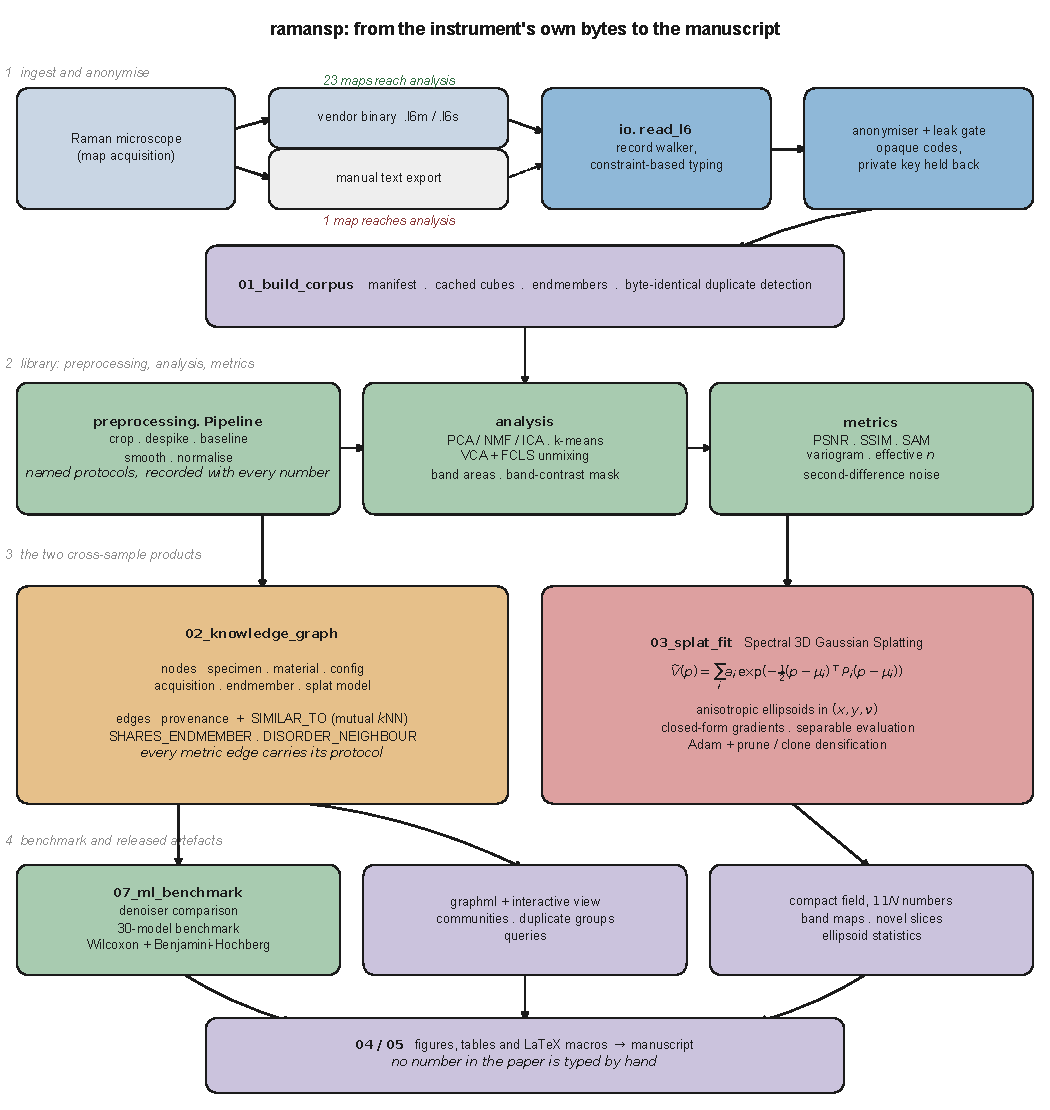
\includegraphics[width=\linewidth]{fig_workflow}
\caption{The \ramansp{} workflow. Reading the vendor container directly
(top, blue) replaces the manual text export that otherwise decides which
measurements reach analysis, taking this study from one hyperspectral map to
\Nrawmap{}. Preprocessing protocols (green) are named and recorded, so every
downstream number travels with the chain that produced it. The two analysis
products, the cross-sample graph (orange) and the Gaussian field (red), consume
the same corpus. The final stage emits every quoted number as a LaTeX macro, so
no figure in the manuscript is typed by hand.}
\label{fig:workflow}
\end{figure*}

\paragraph{Containers.}
\code{Spectrum}, \code{SpectralImage} and \code{SpectralVolume} wrap a
contiguous intensity array together with a shared monotonic wavenumber axis and
a metadata dictionary. The spectral axis is always the last array axis, and is
normalised to ascending order on load so that downstream code never has to test
for orientation. A \code{SpectralImage} may be gridded, shape $(H,W,K)$, or an
unstructured bag of spectra, shape $(N,K)$; the loader decides which, and
refuses to fabricate a grid from coordinates that do not form a clean raster.

\paragraph{Preprocessing.}
A \code{Pipeline} is an ordered list of steps drawn from cropping, despiking,
baseline correction, smoothing and normalisation. Named protocols bundle the
recipes we use: \code{carbon\_dg} (arPLS baseline \cite{baek2015arpls},
then Savitzky and Golay smoothing, then area normalisation), \code{arpls},
\code{chord} and \code{poly3} for straight and polynomial baselines, and
\code{minimal}. The protocol name and its full parameterisation are recorded in
the output metadata, so any number computed downstream travels with the recipe
that produced it.

One implementation note has a large practical consequence. The arPLS system
matrix $\operatorname{diag}(w) + \lambda D^{\!\top}\!D$, with $D$ the
second-difference operator, is symmetric and pentadiagonal. Solving it with a
banded Cholesky factorisation rather than a general sparse solver gives the
same matrix and the same answer to $4\times10^{-11}$ relative difference at
roughly five times the speed. Whole-corpus reprocessing is what makes a
cross-sample study possible at all, and that factor is the difference between
a half-hour job and a three-hour one.

\paragraph{Analysis.}
PCA, NMF and ICA decomposition and $k$-means clustering wrap scikit-learn.
Linear unmixing implements VCA \cite{nascimento2005vca} followed by
fully-constrained least-squares abundances. Carbon band areas are integrated
above local polynomial baselines anchored in windows flanking each band, with a
band-free control window integrated by the identical procedure as an acceptance
test: a correct baseline returns approximately zero there, so the claim is
checkable rather than asserted.

\label{sec:masking}Particle and substrate are separated by an Otsu split on log
total counts, which requires no noise estimate and therefore avoids the
circularity of using a noise threshold to define the mask that defines the
noise. Which side of that split is the particle is then decided
spectroscopically rather than photometrically. The obvious rule, that the
particle is the darker side, is correct for a dark grain on a bright
fluorescent substrate and wrong whenever the contrast runs the other way, which
happens in this corpus. The framework instead compares band contrast, the
height of the carbon bands above a band-free window, across the two sides and
keeps the side that carries the bands. That measure is a shape rather than a
brightness, so it survives normalisation and answers the question actually
being asked, namely which pixels carry Raman signal from the material.

Spatial statistics include the variogram, Moran's $I$ and an
AR(1) effective sample size, so that significance within a map can be quoted at
the number of independent samples rather than the pixel count.

\paragraph{Corpus construction and anonymisation.}
The framework walks a study directory and ingests curve-fit tables,
matrix-format maps and line scans, single spectra, instrument calibration
spectra, and the vendor's proprietary binaries. It writes a compact,
anonymised corpus: one row per acquisition in a manifest, cached arrays for
the spectral data, and a machine-readable summary.

A single-pass scanner assigns opaque codes to every specimen identifier,
material designation, person name and dated session folder, and the forward map
is written to one file under \code{\_private/} and nowhere else. Codes are
required to be genuinely opaque: a code built from the initials of the material
it replaces still discloses that material to any reader who knows the field, so
materials receive sequential labels instead, and the gate described below
rejects initial-bearing codes as leaks in their own right. Two names pass through deliberately,
because glassy carbon and graphite are public reference standards rather than
study identifiers, and naming them is scientifically useful. A separate gate,
\code{run/check\_anonymity.py}, scans every shareable output for identifiers
and exits non-zero on a hit, so the property is enforced rather than intended.
On the study analysed here the result is \Nacq{} acquisitions
(Table~\ref{tab:corpus}).

\begin{table}[t]\centering\small
\caption{Composition of the anonymised corpus.}
\label{tab:corpus}
\IfFileExists{tables/corpus.tex}{\begin{tabular}{lr}
\toprule
acquisition kind & count \\
\midrule
fit table & 40 \\
spectrum & 36 \\
raw map & 23 \\
autocal & 7 \\
raw scan & 2 \\
\midrule
total & 108 \\
\bottomrule
\end{tabular}
}{%
\begin{tabular}{lr}\toprule kind & count\\\midrule fit table & \Nfittable\\
raw map & \Nrawmap\\ raw scan & \Nrawscan\\ \bottomrule\end{tabular}}
\end{table}

% ==================================================================

\subsection{Reading the vendor container}
\label{sec:l6}

Horiba LabSpec\,6 stores maps and spectra in undocumented binaries
(\code{.l6m}, \code{.l6s}). \code{io.read\_l6} reads them directly.

\paragraph{Container layout.}
After an eight-byte \code{LabSpec6} magic and a version word, the file is a
flat table of 24-byte records with the fields
\code{[type][id][tag][ptr\_hi][val][extra]}. A record whose four-byte tag
contains the ASCII \code{mat} is followed, at record start plus 24 bytes, by a
contiguous little-endian \code{float32} array running to the next record.
Several such arrays exist per map: the intensity cube, the wavenumber axis and
the two stage-coordinate axes.

\paragraph{The one trap.}
The \code{ptr\_hi} field looks like a format constant and is not. It is the
high half of a serialised 64-bit Windows pointer, so its value
(\code{0x7ff6}, \code{0x7ff7}, or zero in the 32-bit container variant) records
where the writing process happened to be mapped in memory at save time, and it
differs between files written by the same software on the same machine. Any
parser that hard-codes it works on the file it was developed against and fails
silently on the next one. We calibrate it per file from the bytes following a
known tag, then use it to walk the record table.

\paragraph{Identification by constraint.}
The arrays carry no labels, so the reader identifies them by constraint rather
than by position. The intensity cube is the largest array. The wavenumber axis
is the longest strictly ascending array lying in a plausible Raman-shift range
whose length divides the cube. The two stage axes are the \emph{evenly stepped}
pair whose lengths satisfy $n_x \cdot n_y \cdot K = |\text{cube}|$; the
even-step requirement matters, because intensity data contains ascending runs
by chance and an unconstrained search will happily accept one as an axis and
reshape the cube wrongly. Which stage axis is the outer one is likewise
unlabelled, so both orders are scored by map isotropy: read at the true row
length a map is an isotropic two-dimensional field, and read at the wrong one
the vertical neighbours are unrelated points whose differences inflate. If no
assignment satisfies the constraint, the reader raises rather than guessing.

\paragraph{Verification.}
The corpus contains one map for which both the binary and the instrument's own
text export exist, which makes an exact check possible. The recovered cube is
bit identical to the export, \SI{766080}{} \code{float32} values with zero
differences, and the wavenumber axis, grid dimensions and stage extent all
agree. The binary is in fact the more precise of the two, since the text export
rounds the axis to six significant figures. Independently of that single pair,
across the \Nlsix{} binaries the reader accepts, the mean spectra place the
carbon D and G bands at a median of \SI{1348}{} and
\SI{1580}{\per\centi\metre} respectively, which is where they belong. The first
check establishes that the bytes are decoded correctly; the second establishes
that the result is physically meaningful across files the first check never
saw.

\paragraph{What this buys.}
Fig.~\ref{fig:corpus} is the answer in one picture. Reading the binaries takes
the corpus from \Nrawmaptext{} hyperspectral map available through the
instrument's text exports to \Nrawmap, across \Nacq{} acquisitions in total.
That is the difference between a single-map case study and a cross-sample one,
and every result in this paper that compares maps depends on it. The right-hand
panel also shows what the corpus is spectroscopically: a tight envelope with the
D and G bands where they belong, and a small number of acquisitions that sit
well outside it, which the graph of \S\ref{sec:kg} later separates rather than
averages away.

\begin{figure*}[t]\centering
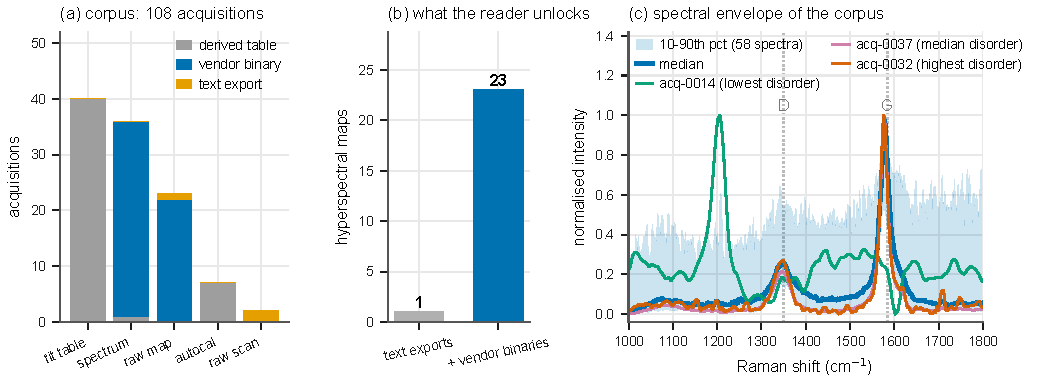
\includegraphics[width=\linewidth]{fig_corpus}
\caption{The anonymised corpus. (a) Composition by acquisition kind, split by
how each file was read. (b) The hyperspectral maps reachable through the
instrument's own text exports against those reachable once the binary container
is decoded. (c) The spectral envelope over every acquisition carrying a
spectrum, each min-max normalised, with the 10th to 90th percentile band, the
median, and the acquisitions at the extremes and the middle of the disorder
index named. Dotted lines mark the nominal D and G positions.}
\label{fig:corpus}
\end{figure*}

\paragraph{Coverage.}
The reader handles the container version that carries the experiment maps. It
does not yet handle an older 32-bit variant that stores its matrices under a
different tag. Those files are overwhelmingly autosave, practice and training
scratch rather than experiments, so the shortfall is in bulk rather than in
scientific content, but it is a real gap and we state it as one
(\S\ref{sec:limitations}).

% ==================================================================

\subsection{Cross-sample knowledge graph}
\label{sec:kgmethod}
\label{sec:kg}

\subsubsection{Motivation}

A Raman study is not a dataset in the machine-learning sense. It is a
heterogeneous accumulation of artefacts: hyperspectral maps, line scans, single
cursor spectra, instrument calibration runs, and curve-fit tables exported from
the vendor software, produced over months, across several specimens, under
several acquisition recipes, by more than one operator. The questions an
experimenter actually asks of such a collection are relational. Which
acquisitions of different specimens share a spectral signature? Does the
disorder metric cluster by material or by acquisition recipe, and if by recipe
then the apparent chemistry is an artefact? Are two files the same measurement
saved twice? Which map should be reanalysed when a calibration run fails?

None of these is answerable one file at a time, and none is naturally expressed
as a table, because the objects are of different kinds and the relations are of
different kinds. A property graph is the appropriate structure, and building
one also forces the metadata discipline that makes the rest of the analysis
trustworthy: an edge cannot be created without deciding what it means and under
what preprocessing it was computed.

\subsubsection{Schema}

\begin{table}[t]\centering\small
\caption{Graph schema. Provenance edges are derived from anonymised paths;
content edges are computed from the data and carry the protocol under which
they were computed.}
\label{tab:schema}
\small
\footnotesize
\begin{tabular}{@{}ll@{}}
\toprule
\textbf{Node type} & \textbf{Represents} \\
\midrule
\code{specimen}    & a physical sample, opaque code \\
\code{material}    & a material or reference class \\
\code{config}      & an acquisition configuration \\
\code{acquisition} & one exported artefact \\
\code{endmember}   & a VCA component of one map \\
\code{splatmodel}  & a fitted Gaussian field \\
\midrule
\textbf{Edge type} & \textbf{Semantics} \\
\midrule
\code{HAS\_ACQUISITION} & specimen produced acquisition \\
\code{OF\_MATERIAL}     & specimen is of material class \\
\code{USED\_CONFIG}     & acquisition used configuration \\
\code{HAS\_ENDMEMBER}   & map decomposes into component \\
\code{MODELLED\_BY}     & map has a fitted field \\
\code{SIMILAR\_TO}      & mutual $k$NN in spectral space \\
\code{SHARES\_ENDMEMBER} & matched component, two specimens \\
\code{DISORDER\_NEIGHBOUR} & close on a stamped metric \\
\bottomrule
\end{tabular}
\end{table}

Nodes and edges are summarised in Table~\ref{tab:schema}. Provenance edges are
recovered from the anonymised directory structure. Content edges are computed:

\begin{itemize}\itemsep2pt
\item \code{SIMILAR\_TO}, a mutual $k$-nearest-neighbour edge with $k=5$,
computed on the mean spectrum resampled to a common axis where spectra exist,
and on a $z$-scored feature vector otherwise. The two bases are never ranked
against each other, because they are not on a common scale and mixing them
would let a curve-fit table outrank a real spectrum. The tabular basis is
flagged \code{confidence=low}, since such a table carries only two of the five
carbon bands and no coordinates.
\item \code{SHARES\_ENDMEMBER}, cosine at least $0.9$ between VCA endmembers
\cite{nascimento2005vca} belonging to \emph{different} specimens. This is the
edge that expresses a chemical claim rather than a similarity of averages: two
specimens may have quite different mean spectra and still contain a common
component.
\item \code{DISORDER\_NEIGHBOUR}, acquisitions within $0.06$ on the bounded
disorder index $A_{D1}/(A_{D1}+A_{G+D2})$ \emph{and} sharing a preprocessing
protocol. The protocol condition is not a formality. As
\S\ref{sec:prep-variance} sets out, a band ratio without its chain is
underspecified, so an edge joining two numbers computed under different chains
would assert a similarity that the data does not support.
\end{itemize}

\subsubsection{Why mutual $k$NN rather than a similarity threshold}

An absolute cosine cut is the obvious construction and the wrong one here.
Every acquisition in this corpus is carbonaceous and therefore has D and G
bands, so spectra are similar almost by construction. Over all pairs the median
cosine is $0.80$, with quartiles at $0.55$ and $0.92$; a cut at $0.65$ links
two thirds of all pairs. The resulting graph has communities and a respectable
modularity, and they describe the threshold rather than the samples.

Fig.~\ref{fig:kgsim} shows what that looks like. The block of acquisitions
that carry real spectra is almost uniformly near unit similarity, so within
that block a threshold anywhere below saturation admits nearly every pair and
anywhere above it admits nearly none. There is no setting that separates them,
which is the situation a threshold cannot survive.

A mutual $k$NN rule asks a relative question instead: are these two
acquisitions among each other's nearest neighbours? It is invariant to a
monotone rescaling of the similarity, keeps average degree bounded by
construction, and degrades gracefully in exactly the regime that defeats a
threshold, namely when everything is somewhat similar to everything else. The
diagnostic that exposed the problem was simply plotting the distribution of
pairwise similarity before choosing a rule rather than after, which we
recommend as routine.


\subsection{Spectral 3D Gaussian Splatting}
\label{sec:s3dgs}

\subsubsection{Representation}

Let the map be sampled on a regular grid and rescaled to the unit cube, with
position $p=(x,y,z)$ where $z$ is the normalised wavenumber. The field is a sum
of $N$ anisotropic three-dimensional Gaussians,
\begin{equation}
\widehat{V}(p)=\sum_{i=1}^{N} a_i\,
\exp\!\Big(-\tfrac12\,(p-\mu_i)^{\!\top} P_i\,(p-\mu_i)\Big),
\label{eq:field}
\end{equation}
with centre $\mu_i\in\mathbb{R}^3$, amplitude $a_i=e^{\lambda_i}>0$, and
precision
\begin{equation}
P_i = R(q_i)\,\operatorname{diag}(s_i^{-2})\,R(q_i)^{\!\top},
\qquad s_i = e^{\ell_i}\in\mathbb{R}^3_{>0},
\end{equation}
where $R(q_i)$ is the rotation of the unit quaternion $q_i$. Each primitive
carries $3+3+4+1 = 11$ parameters. Amplitude and scale are parameterised
logarithmically so that positivity is structural rather than enforced.

Each Gaussian is a genuine ellipsoid in $(x,y,\nu)$. Its two spatial semi-axes
localise a chemical domain, and its wavenumber centre and semi-axis localise a
band and its width. A carbon particle is therefore reconstructed by ellipsoids
clustered over the particle footprint, narrow along $z$, centred near the D and
G positions of the standard assignment \cite{sadezky2005carbon}, with $a_i$
the band intensity. This is what makes the representation legible: a primitive
reads directly as ``a band, at this position, this strong, this wide''.

We are careful about what that does not mean. The ellipsoids are band
\emph{localisers}, not a five-component chemical decomposition. Which defect
populations a $\mathrm{D/G}$ ratio reflects depends on excitation and defect
type \cite{cancado2017disorder}, and a reconstruction of one cube cannot
settle that attribution.

\subsubsection{Objective and analytic gradients}

With residual $r(p)=\widehat V(p)-V(p)$ on the masked voxels $\Omega$,
\begin{equation}
\mathcal{L}=\tfrac12\!\sum_{p\in\Omega}\! r(p)^2
+\lambda_a\!\sum_i a_i
+\lambda_s\!\sum_i \lVert \ell_i\rVert^2 .
\end{equation}
The $L_1$ term on amplitude drives redundant primitives towards zero so that
pruning has something to remove; the term on $\ell$ discourages degenerate
widths.

Writing $d = p-\mu_i$, $\phi_i(p)=\exp(-\tfrac12 d^\top P_i d)$ and
$w = r\,\phi_i$, every gradient is closed form:
\begin{align}
\partial_{\lambda_i}\mathcal L &= a_i\!\sum_p w + \lambda_a a_i,\\
\partial_{\mu_i}\mathcal L &= a_i\!\sum_p w\,(P_i d),\\
M_i \equiv \partial_{P_i}\mathcal L &= -\tfrac{a_i}{2}\!\sum_p w\, d\,d^\top,
\end{align}
and, chaining $P_i=R\Lambda R^\top$ with $\Lambda=\operatorname{diag}(s_i^{-2})$,
\begin{align}
\partial_{\ell_{i,k}}\mathcal L &= -\frac{2}{s_{i,k}^2}\,\big(R^\top M_i R\big)_{kk}
  + 2\lambda_s \ell_{i,k},\\
\partial_{R}\mathcal L &= 2\,M_i R \Lambda,\\
\partial_{q_i}\mathcal L &= \frac{I-\hat q_i\hat q_i^\top}{\lVert q_i\rVert}
  \sum_k \big\langle \partial_R\mathcal L,\  \partial_{\hat q_{i,k}}R\big\rangle ,
\end{align}
the last factor propagating through the normalisation $\hat q = q/\lVert q
\rVert$. Every expression is validated against central finite differences to a
relative error below $10^{-4}$, as a unit test rather than as a one-off check,
so a later optimisation cannot silently break the mathematics.

\subsubsection{Optimisation and complexity}
\label{sec:optimisation}

\begin{algorithm}[t]
\caption{S3DGS fit (pure NumPy)}\label{alg:fit}
\begin{algorithmic}[1]
\State importance-sample $N$ centres with probability $\propto |V|$
\State initialise $s$ at a fixed voxel width, $q$ at identity
\For{$t=1,\dots,T$}
  \State $\widehat V \gets$ Eq.~\eqref{eq:field} on each primitive's $3\sigma$ box
  \State $\mathcal L,\nabla \gets$ closed-form gradients (\S5.2)
  \State Adam step \cite{kingma2015adam} with per-group rates
  \State clamp $\ell$ to the permitted width range, in voxels
  \If{$t \bmod \tau = 0$ and $t \le T/2$}
    \State clone or split primitives with large $\lVert\partial_\mu\mathcal L\rVert$
    \State prune primitives with $a_i < \epsilon\,\mathrm{median}(a)$
  \EndIf
\EndFor
\end{algorithmic}
\end{algorithm}

Every fifth wavenumber channel is withheld from $\Omega$ and used only for
scoring. Quality is reported as PSNR, SSIM \cite{wang2004ssim}, spectral angle,
and the noise-floor ratio introduced in \S\ref{sec:results}.

Three implementation decisions determine whether this is practical.

\emph{Truncation.} Each Gaussian is evaluated only on the grid voxels inside
its $3\sigma$ box. Cost is therefore $O(N \cdot B)$ per iteration with $B$ the
box volume in voxels, independent of the size of the map, which is why a
$153\times144$ map costs about what a $30\times32$ map costs at the same
primitive count. The whole population is advanced as one batched array
expression \cite{harris2020numpy} rather than a Python loop over primitives.

\emph{Locating the box by search.} The box must be centred by searching the
axis, not by dividing by a nominal spacing. The fitted wavenumber axis is not
uniformly spaced once every fifth channel is withheld, and the drift that
results from assuming otherwise is the subject of \S\ref{sec:pitfalls}.

\emph{Separable evaluation.} The quadratic form expands as
\begin{equation}
d^{\!\top}\! P d = \sum_{k} P_{kk} d_k^2 + 2\!\!\sum_{k<l}\!\! P_{kl} d_k d_l ,
\end{equation}
and each offset $d_k$ depends on only one box axis. The
$(N, B_y, B_x, B_z, 3)$ offset tensor, which reaches hundreds of megabytes for
a few thousand primitives, is therefore never formed, and every gradient
contraction reduces to nine scalars per primitive: three first moments for
$\partial_\mu$ and six second moments for $M_i$.

Primitive widths are bounded in voxels rather than in absolute units. This
keeps the box volume, and hence the cost, constant across maps of very
different pixel counts, and it keeps the meaning of a primitive constant too:
a primitive should not be much wider than the sampling that produced it.

\begin{table}[t]\centering\small
\caption{Fitting hyperparameters. Learning rates are per parameter group, in
the convention of \cite{kerbl20233dgs}, where centres must move far more slowly
than amplitudes. The primitive count is set from the masked volume so that
density rather than count is held approximately fixed across maps.}
\label{tab:hyper}
\begin{tabular}{@{}lll@{}}
\toprule
symbol & value & meaning \\
\midrule
$T$              & 140              & iterations \\
hold-out         & every 5th        & withheld channels \\
bin              & 4                & wavenumber binning \\
$\eta_\mu$       & $4\times10^{-4}$ & centre rate \\
$\eta_\ell$      & $6\times10^{-3}$ & log-scale rate \\
$\eta_q$         & $3\times10^{-3}$ & quaternion rate \\
$\eta_\lambda$   & $3\times10^{-2}$ & log-amplitude rate \\
$\lambda_a$      & $2\times10^{-4}$ & amplitude $L_1$ \\
$\lambda_s$      & $1\times10^{-4}$ & scale prior \\
trunc            & $3\sigma$        & evaluation radius \\
$s$ bounds       & 0.45 to 2.6 vox  & primitive width \\
$\tau$           & 40               & densify interval \\
densify until    & $T/2$            & no growth after \\
prune            & $5\times10^{-3}\bar a$ & amplitude floor \\
\bottomrule
\end{tabular}
\end{table}

\subsubsection{Scaling to millions}
\label{sec:scale}
The NumPy engine is demonstrated at $10^3$ primitives and is expected to reach
$10^4$ to $10^5$ on a CPU. The port to the $10^6$ to $10^7$ regime is the
standard tiled rasteriser \cite{kerbl20233dgs} with a third axis: parameters
become CUDA tensors and automatic differentiation replaces \S5.2, with the
closed-form gradients retained as the test oracle; the volume is partitioned
into $16^3$ voxel tiles and each primitive is assigned by segmented sort to the
tiles its $3\sigma$ box intersects, so each tile sums only its own primitives;
and densification runs over the full population every hundred steps. An
optional extension gives each primitive a length-$D$ code over an NMF or VCA
endmember dictionary $\Phi$, so that the field value becomes $\sum_i a_i
G_i(p)\,(\Phi^\top c_i)(\nu)$ and every ellipsoid carries a physically
realisable Raman profile rather than a scalar amplitude.

% ==================================================================

% ==================================================================
\section{Results and Discussion}
\label{sec:results}

\subsection{Reconstruction of hyperspectral maps}

\paragraph{Setup.}
All fits run single-threaded on a CPU, in double precision, with no GPU.
The flagship map is \SplatAcq{}: $\SplatMapNy\times\SplatMapNx$ pixels and
\SplatMapK{} channels, restricted to its \SplatMaskPts{} particle pixels by an
Otsu split on log counts. Wavenumber channels are binned by four before
fitting, and every fifth surviving channel is withheld.

\paragraph{Flagship reconstruction.}
S3DGS fits \SplatN{} ellipsoids in \SplatSeconds{} seconds. Reconstruction
reaches \SplatPSNRtrain\,dB PSNR on fitted channels and \SplatPSNReval\,dB on
withheld channels, with SSIM \SplatSSIM{} on band maps and a mean spectral
angle of \SplatSAM{} rad. Because the field is continuous in $\nu$, it stands
in for the full-resolution cube: \SplatParams{} stored numbers replace
\SplatRawValues{} masked cube values, a \SplatCompression$\times$ reduction, or
\SplatCompressionBinned$\times$ counted only against the binned channels the
fit actually saw. Band maps rendered from the field reproduce the integrated
band-area maps (Fig.~\ref{fig:bands}), and per-pixel spectra including withheld
channels are recovered (Fig.~\ref{fig:spectra}).

The primitives also organise themselves, and Fig.~\ref{fig:ellipsoids} is the
evidence for the two claims the representation rests on. The first is that the
anisotropy is used: the median ratio of longest to shortest semi-axis is
\SplatAniso, so a typical primitive is a flattened disc rather than a ball, and
the strongest are wide in $x$ and $y$ and thin along $\nu$. That is the
geometry one would draw by hand for a Raman band, and it was not imposed. The
second is that the amplitude lands on the bands: \SplatAmpBands\,\% of the total
amplitude belongs to primitives whose centre lies inside the D1 or G+D2 window,
although those two windows together cover only \SplatBandSpan\,\% of the fitted
wavenumber range. Nothing in the loss refers to band positions, so the
concentration is a property of the data recovered by the fit rather than a
constraint satisfied by it.

\paragraph{Across maps, and what actually limits the fit.}
Fitting \SplatNfits{} maps spanning different acquisition recipes gives
held-out PSNR from \SplatPSNRevalMin{} to \SplatPSNRevalMax\,dB at
\SplatComprMin{} to \SplatComprMax$\times$ compression
(Table~\ref{tab:splat}). Read naively that is a wide and unflattering spread.
It is also the wrong reading, and the reason is worth stating plainly:
\textbf{PSNR against a measured target confounds the representation with the
measurement}. These acquisitions differ in exposure, and the signal-to-noise
of the maps themselves spans \SplatSNRmin{} to \SplatSNRmax, measured on each
map by the same second-difference estimator used below.

Fig.~\ref{fig:quality} shows the confound rather than asserting it. Against
primitive budget, held-out PSNR has no usable trend: the map with the second
largest budget scores worst. Against each map's own signal-to-noise it lines up
at Pearson $r=\SplatPSNRSNRr$. The quantity the spread in PSNR is mostly
reporting is therefore how noisily each map was measured.

The honest comparison is the held-out residual against an \emph{independent}
estimate of each map's own noise, obtained from second differences along
wavenumber, since a band spans tens of channels and noise does not. That ratio
$r/\sigma$ runs from \SplatResidNoiseMin{} to \SplatResidNoiseMax{} across the
set (Fig.~\ref{fig:quality}c). \SplatNatFloor{} of \SplatNfits{} maps sit at or
below their own noise floor and \SplatNnearFloor{} sit within
\SI{\SplatFloorBand}{\percent} of it, which is possible only because a smooth
field of ellipsoids cannot represent white noise and therefore discards it. The low-PSNR maps are not badly reconstructed. They are noisily
measured, and the field is declining to fit the noise.

That interpretation is testable and we test it, on synthetic data where the
clean signal is known: a field fitted to a noisy cube ends up closer to the
underlying clean signal than the noisy cube it was fitted to. The property is
kept as a unit test rather than a figure.

\paragraph{A caveat we do not paper over.}
The primitive budget is capped, so density $\rho$ is not constant across the
set, running from \SplatRhoMin{} to \SplatRhoMax{} primitives per 1000 voxels,
and the larger maps are the more thinly parameterised. Quality does track
$\rho$ (Fig.~\ref{fig:quality}, left), with the noisiest map as the clear
outlier, exactly as the noise-floor account predicts. A clean rate-distortion
study would sweep $\rho$ on a single map rather than inferring the trend across
maps of differing difficulty, and we flag that as the correct next experiment
rather than claiming the present one substitutes for it.

\begin{table}[t]\centering\small
\caption{S3DGS across acquisitions. $\rho$ is primitives per 1000 fitted
voxels; PSNR is on wavenumber channels withheld from the fit; $r/\sigma$ is
that residual over the map's own measurement noise, where $1.0$ is the noise
floor.}
\label{tab:splat}
\IfFileExists{tables/splat.tex}{\begin{tabular}{lrrrrr}
\toprule
map & $N$ & $\rho$ & compr. & PSNR (dB) & $r/\sigma$ \\
\midrule
map 0042 & 2912 & 12 & 38.0 & 22.5 & 1.06 \\
map 0039 & 2912 & 13 & 36.2 & 22.9 & 1.02 \\
map 0028 & 2912 & 13 & 34.5 & 16.9 & 1.12 \\
map 0059 & 2912 & 15 & 29.6 & 19.1 & 1.09 \\
map 0016 & 2912 & 24 & 19.1 & 10.9 & 1.43 \\
map 0055 & 1239 & 56 & 8.1 & 27.2 & 0.70 \\
\bottomrule
\end{tabular}
}{%
\begin{tabular}{lrrrrr}\toprule map & $N$ & $\rho$ & compr. & PSNR (dB) & $r/\sigma$\\\midrule
n/a & n/a & n/a & n/a & n/a & n/a\\\bottomrule\end{tabular}}
\end{table}

\begin{figure*}[t]\centering
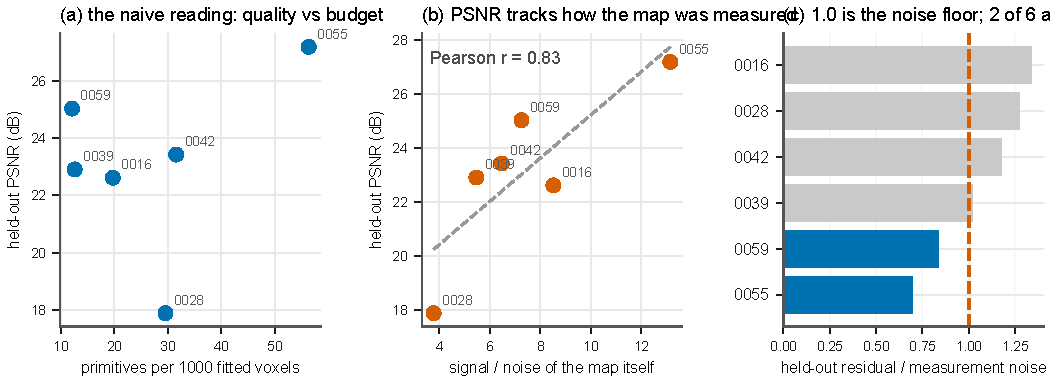
\includegraphics[width=\linewidth]{fig_splat_quality}
\caption{Why held-out PSNR is the wrong headline number across maps. (a)
Against primitive budget there is no usable trend. (b) Against each map's own
signal-to-noise, measured from second differences along wavenumber, the same
points line up: PSNR is largely reporting how the map was measured rather than
how well it was represented. (c) The measure that does not have that defect,
namely the held-out residual divided by that same independent noise estimate.
The dashed line at $1.0$ is the noise floor; a bar at or below it means the
field is no further from the data than the data is from itself, and a bar
below it means the field is declining to reproduce noise.}
\label{fig:quality}
\end{figure*}

\begin{figure*}[t]\centering
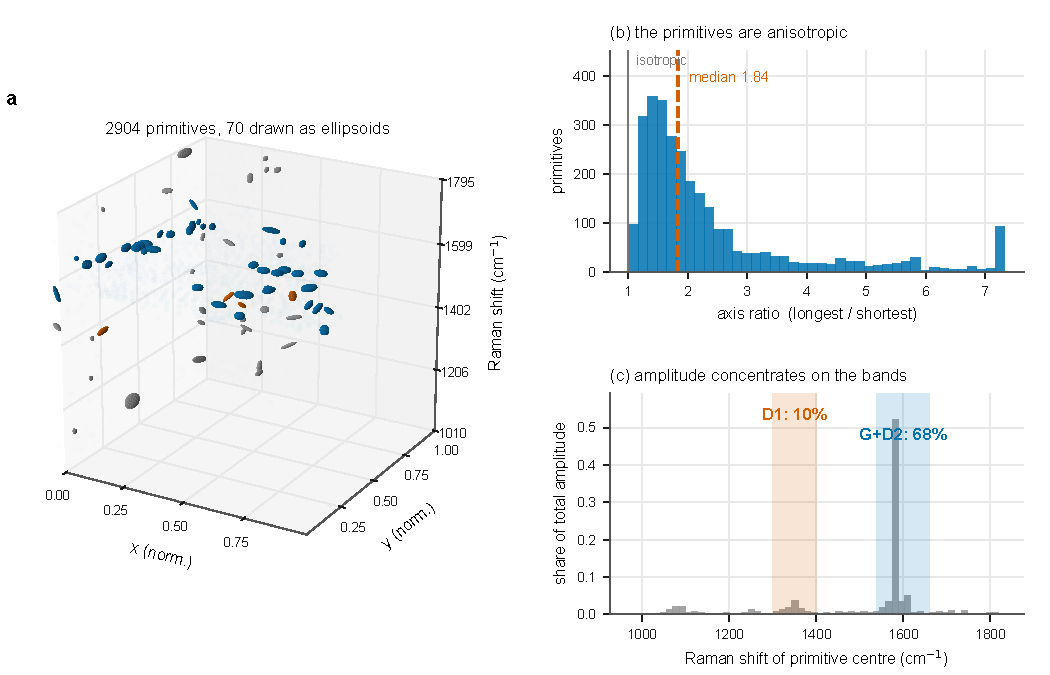
\includegraphics[width=\linewidth]{flagship_ellipsoids}
\caption{What the fitted field is made of. (a) The strongest primitives drawn
as true ellipsoid surfaces from their own covariance, in the normalised cube
the model is optimised in, so the shapes on the page are the shapes in the fit.
Colour marks the carbon band a primitive's centre falls in, and the remaining
centres are faint dots. The band primitives are discs, wide in the two spatial
axes and thin along wavenumber, which is the geometric statement that a band
sits at one Raman shift and extends over a region of the specimen. (b) The
distribution of axis ratios, confirming the anisotropy is used rather than
merely permitted. (c) Where the amplitude goes: the share of total amplitude
whose primitive centre lies inside each carbon band window. The concentration
is a result, not a constraint, since nothing in the loss refers to band
positions.}
\label{fig:ellipsoids}
\end{figure*}

\begin{figure}[t]\centering
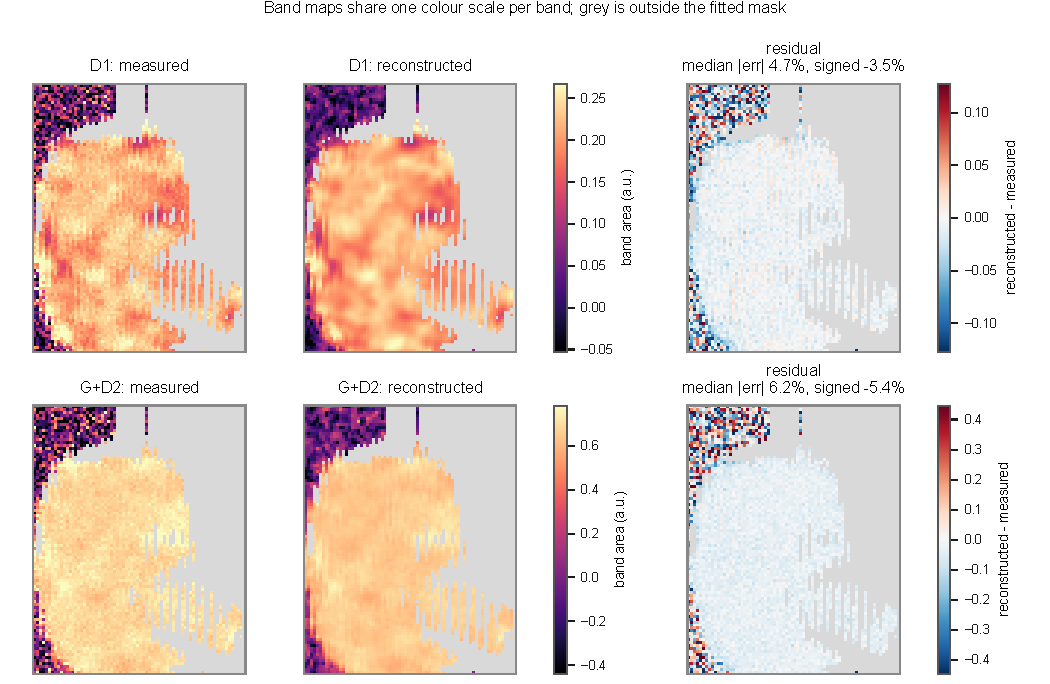
\includegraphics[width=\linewidth]{flagship_bands}
\caption{Measured integrated band-area maps (top) against the same bands
rendered from the Gaussian field (bottom), for $D1$ and $G{+}D2$.}
\label{fig:bands}
\end{figure}

\begin{figure}[t]\centering
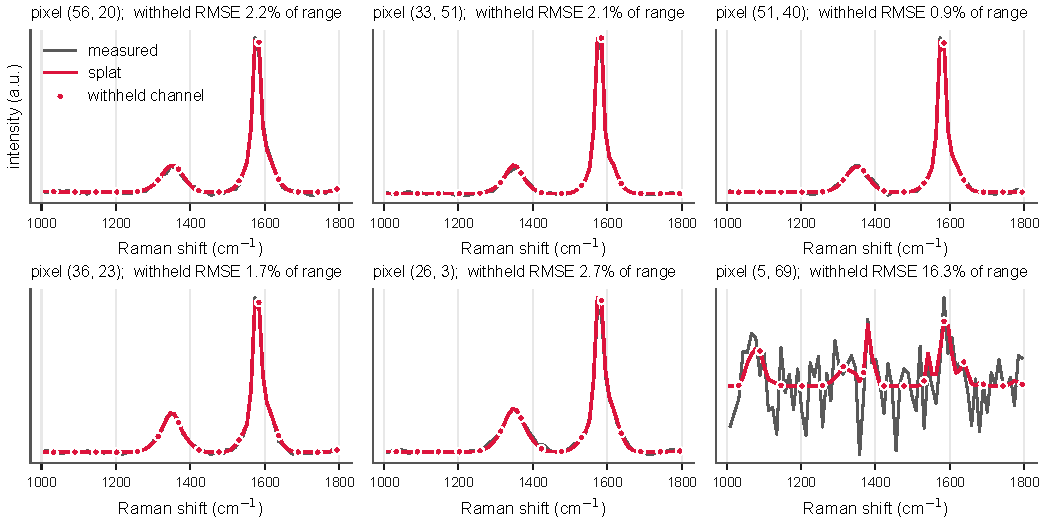
\includegraphics[width=\linewidth]{flagship_spectra}
\caption{Measured (grey) against reconstructed (red) spectra at random particle
pixels. Dots mark the withheld wavenumber channels, which the field never saw
during fitting, and each panel reports the root-mean-square error on those
channels as a percentage of that pixel's measured range. The comparison to make
is not how smooth the red curve is but how close the dots land, since the
smoothness is free and the dots are not.}
\label{fig:spectra}
\end{figure}

\paragraph{Preprocessing dependence.}
A disorder number is only worth carrying on a graph edge if it survives the
baseline choice, and that is a comparison rather than a measurement, so
Fig.~\ref{fig:ablation} asks it of both candidates at once. Each of
\AblNmaps{} maps is preprocessed under \AblNproto{} baseline families, and each
contributes one paired trace, since the question is whether a protocol moves a
given map rather than whether maps differ. The \AblNmaps{} are the smallest maps
in the corpus by masked point count, and up to 900 in-mask spectra are drawn
from each; both limits are there to keep five full preprocessing chains
affordable, and neither is chosen with reference to the result.

The separation is not marginal. The bounded index
$A_{D1}/(A_{D1}+A_{G+D2})$ moves by a median of
\SI{\AblSpreadMedian}{\percent} of a map's own value across the five
protocols, and by at most \SI{\AblSpreadMax}{\percent} on the worst map. The
raw peak-height ratio $I_D/I_G$ computed on the same spectra under the same
five protocols moves by a median of \SI{\AblSpreadRaw}{\percent}, more than an
order of magnitude further, and its traces cross: the protocol can reorder two
maps. A ratio that can be reordered by a baseline choice cannot support an edge
asserting that two samples are alike, and that is the concrete reason the
bounded index is what the graph carries. It is also why the protocol is
recorded on every \code{DISORDER\_NEIGHBOUR} edge even so, because
\SI{\AblSpreadMax}{\percent} on the worst map is not zero.

\begin{figure*}[t]\centering
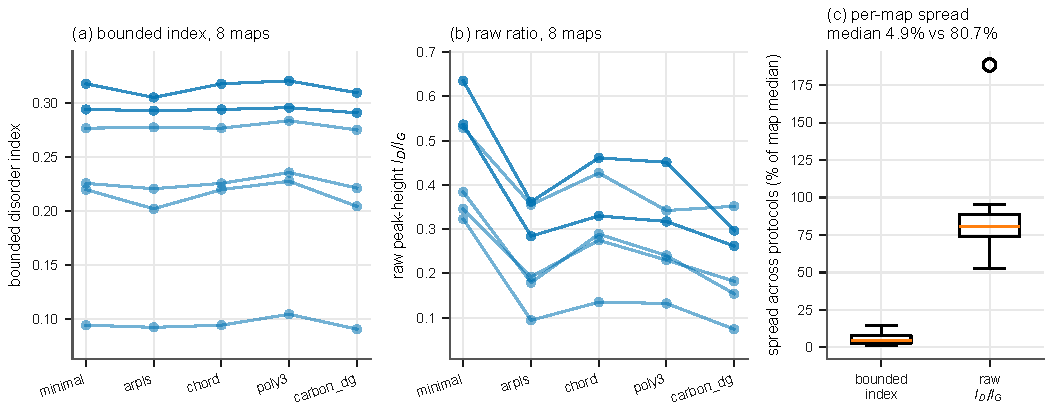
\includegraphics[width=\linewidth]{fig_preproc_ablation}
\caption{Stability of two disorder measures under the baseline choice, over
\AblNmaps{} maps and \AblNproto{} preprocessing protocols. (a) The bounded
disorder index; each line is one map, and the lines are close to flat. (b) The
raw peak-height $I_D/I_G$ on the same spectra under the same protocols; the
lines swing and cross, so the protocol can change which map looks more
disordered. (c) The per-map spread across protocols, expressed as a percentage
of that map's own median, for the two measures. Axes in (a) and (b) are scaled
to their own data rather than to zero, since the comparison is between the two
spreads and a zero baseline would hide both.}
\label{fig:ablation}
\end{figure*}

% ==================================================================

\subsection{Structure recovered by the knowledge graph}
\subsubsection{Community structure and interpretation}

Communities are extracted by greedy modularity maximisation over the content
sub-graph only, so that provenance edges, which are true by construction,
cannot manufacture structure. On this corpus the graph has \KGnodes{} nodes and
\KGedges{} edges in \KGcommunities{} communities at modularity
$Q=\KGmodularity$ (Table~\ref{tab:kg}, Fig.~\ref{fig:kg}), with purity against
the sparse material labels of \KGpurity{}.

Three results are worth separating from the summary statistics.

\emph{Duplicate detection.} The graph flags \Ndupgroups{} groups of
byte-identical curve-fit exports, the same measurement saved repeatedly under
different names. This matters beyond tidiness: undetected, such duplicates
inflate every count-based statistic over the corpus and, in a
similarity-clustered analysis, create artificially tight clusters that invite
interpretation as reproducibility.

\emph{Connectivity depends on the reader.} With text exports alone the graph
falls into two disconnected components, a small provenance-linked cluster and a
large decontextualised dump of curve-fit tables with no specimen or
configuration attached. Reading the vendor binaries (\S\ref{sec:l6}) collapses
this to essentially one connected object, because the binaries carry the
provenance the exports discard. The change is qualitative, not a matter of
degree, and it illustrates the argument of \S1(ii): what a corpus appears to
contain is a property of the reader as much as of the experiment.

\emph{What the communities are not.} Purity of \KGpurity{} against material
labels is computed over a small number of labelled acquisitions and should be
read as a description of what the method surfaces on this corpus, not as
evidence that these materials separate. We return to this in
\S\ref{sec:limitations}.

\subsubsection{Queries}

The graph is written as GraphML and is intended to be queried rather than only
plotted. Representative traversals include: all acquisitions of a specimen
sharing an endmember with a different specimen; acquisitions whose disorder
index is close under one protocol but not under another, which localises
protocol sensitivity to particular samples; maps that have a fitted field and
therefore a compact reconstruction available; and configurations whose
acquisitions cluster together, which is the signature of an acquisition
artefact rather than a chemical one. This last query is the reason
\code{config} is a first-class node: separating chemistry from recipe is only
possible if the recipe is in the graph.

\begin{table}[t]\centering\small
\caption{Knowledge-graph summary.}\label{tab:kg}
\IfFileExists{tables/kg.tex}{\begin{tabular}{lr}
\toprule
quantity & value \\
\midrule
nodes & 236 \\
edges & 636 \\
communities & 23 \\
modularity $Q$ & 0.65 \\
community purity vs.\ class & 0.86 \\
\bottomrule
\end{tabular}
}{%
\begin{tabular}{lr}\toprule quantity & value\\\midrule nodes & \KGnodes\\
edges & \KGedges\\ communities & \KGcommunities\\ modularity $Q$ & \KGmodularity\\
\bottomrule\end{tabular}}
\end{table}

\begin{figure*}[t]\centering
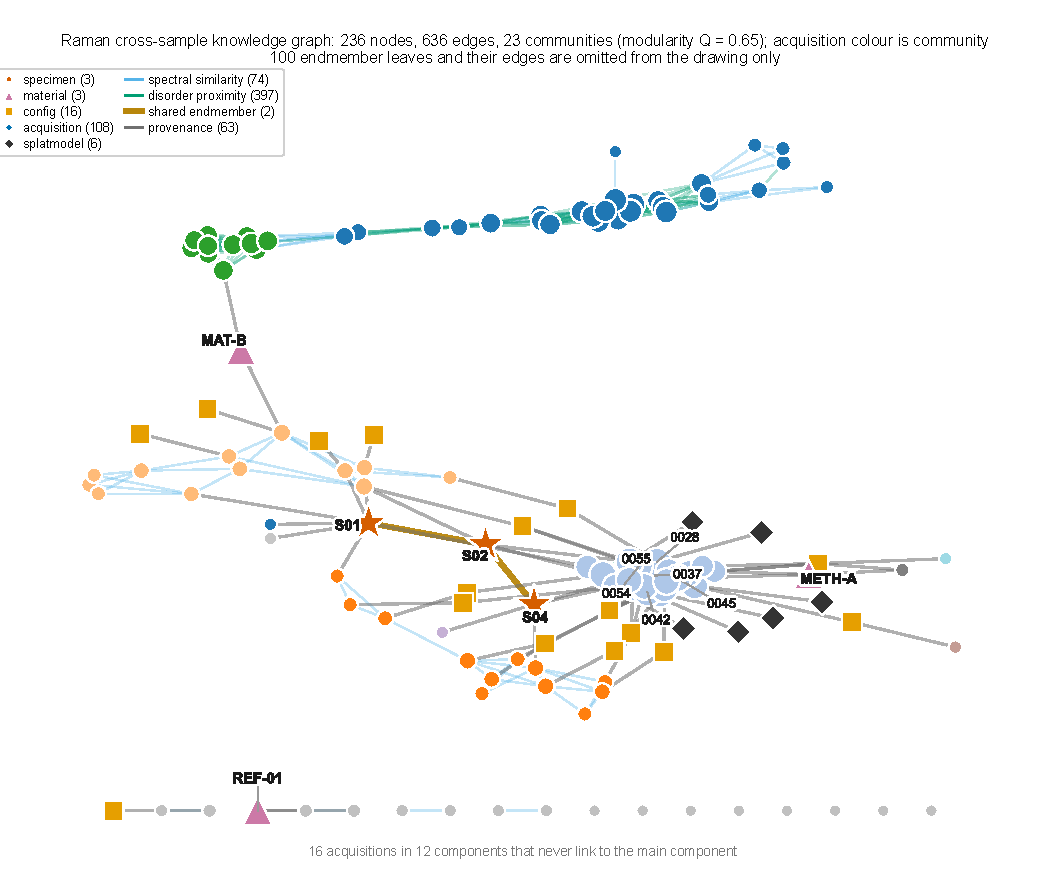
\includegraphics[width=\linewidth]{kg_graph}
\caption{The cross-sample knowledge graph. Node type is encoded by marker and
acquisitions are coloured by detected community. Provenance edges are the grey
backbone that ties acquisitions to their configuration, material and specimen;
the coloured edges are content edges that were earned from the data. Endmember
leaves are omitted from the drawing, since there are four per map and each
attaches to exactly one acquisition, so they inflate the node count without
adding connectivity; the reported node and edge counts are for the full graph.
Components that never reach the main component are parked in the strip below,
and their presence is the point: not every acquisition earns a content link,
and a graph that connected everything would be measuring its own threshold
rather than the corpus.}
\label{fig:kg}
\end{figure*}

\begin{figure*}[t]\centering
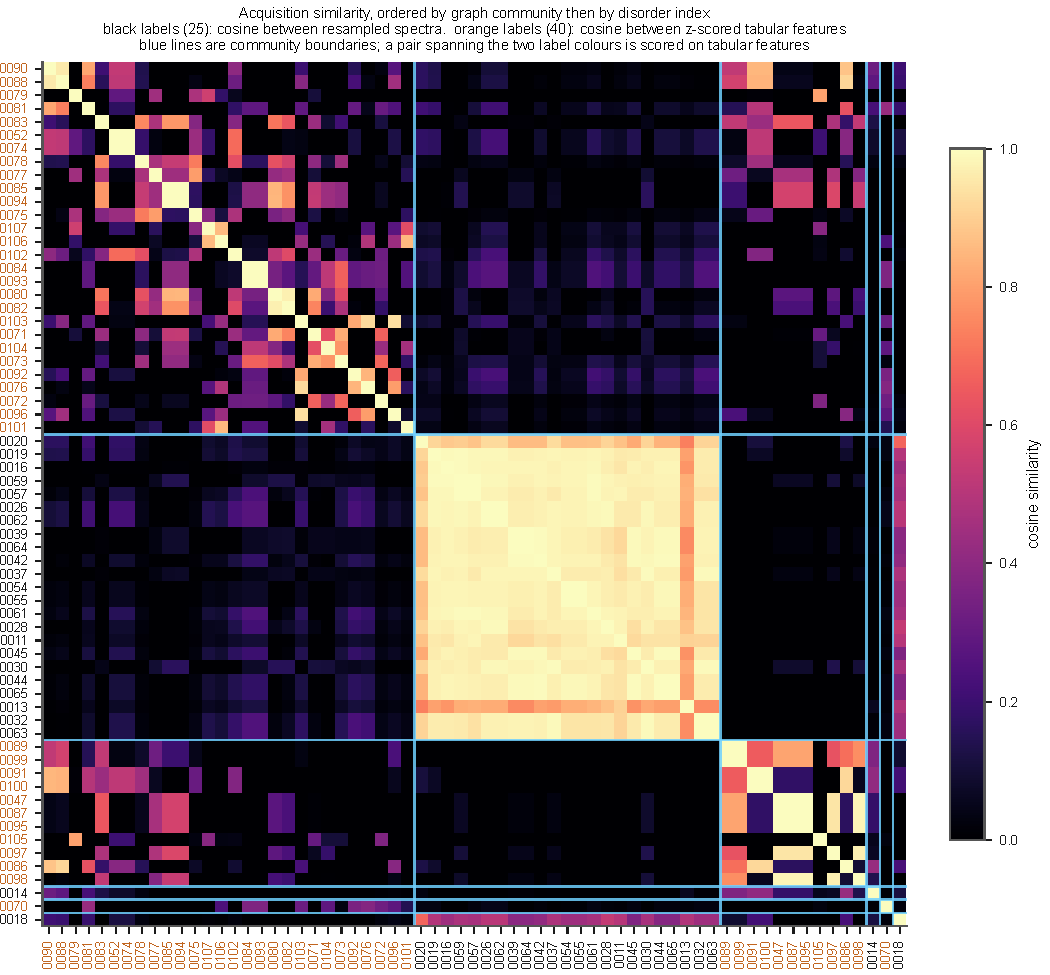
\includegraphics[width=\linewidth]{kg_similarity_heatmap}
\caption{Pairwise acquisition similarity, ordered by detected community and
then by disorder index, with community boundaries drawn. Label colour records
which quantity produced each row, because the matrix is not homogeneous: pairs
that both carry a spectrum are compared by cosine between resampled spectra,
and every other pair falls back to cosine between standardised tabular
features. The block of near-unit similarity among the spectral acquisitions is
the reason a fixed cosine threshold is not usable on this corpus, and the
empirical motivation for the mutual $k$-nearest-neighbour rule of
\S\ref{sec:kg}. Presenting the two measures on one colour scale without marking
which is which would invite exactly the comparison the data does not support.}
\label{fig:kgsim}
\end{figure*}

% ==================================================================

\subsection{Benchmarking against the standard toolkit}
\label{sec:benchmark}

A framework that adds a representation should be measured against the methods
it hopes to sit beside. We report two benchmarks. Both run on this corpus
rather than on published data: the reference datasets used in comparable
studies are not distributed with this work, so we reproduce the experimental
\emph{designs} and report our own numbers rather than quoting theirs.

\subsubsection{Denoising}

Following the paired design used for held-out denoiser evaluation, the
highest contrast-to-noise map in the corpus is contaminated with additive
Gaussian noise to form the input, and the original serves as the target. We
compare six Savitzky-Golay filters \cite{savitzky1964smoothing} spanning
polynomial orders 2 to 5 and kernels 5 to 25, a PCA rank-truncation denoiser
truncated at the Marchenko-Pastur noise edge, and the fitted Gaussian field
used as a denoiser, on three metrics in common use: mean squared error,
spectral angle distance \cite{kruse1993spectral} and spectral information
divergence \cite{chang1999spectral}. Significance is a two-sided Wilcoxon
signed-rank test over spectra against the best-performing Savitzky-Golay
filter, with Benjamini-Hochberg correction for the resulting family of
comparisons \cite{benjamini1995controlling}.

Every method sees the same corrupted map. In particular the two that pool
information across spectra, PCA truncation and the Gaussian field, are fitted
to the whole contaminated cube and then read back at the scored spectra, and
the field is given the same primitive density the rest of this study uses
rather than a reduced budget, so the comparison is of methods as deployed.

Results are in Fig.~\ref{fig:mldenoise} and Table~\ref{tab:mldenoise}. The
clearest effect is that kernel width dominates the Savitzky-Golay family: the
shortest kernel is the best of them by a wide margin, and the longest is worse
than leaving the data alone, because the carbon bands are narrow enough that a
wide polynomial window removes signal along with noise. This is the
preprocessing-sensitivity argument of \S\ref{sec:prep-variance} reappearing in
a different guise, and it is why the comparison runs across a family of filters
rather than against one arbitrarily chosen setting. Reporting against a single
mid-range filter would have made every other method look better than it is.

On this task the ranking does not favour our own representation, and we report
it as measured. The best method overall is \MLBestDenoiser, which improves mean
squared error over the untouched input by \MLDenoiseGain$\times$, and the best
Savitzky-Golay filter is \MLRefFilter; the Gaussian field does not
beat the input at all on that metric. Raising its budget from a token
allocation to \MLSplatRho{} primitives per 1000 voxels improved it but did not
change the ordering, so this is a property of the model rather than of the
budget it was given. A field fitted to a whole map optimises a global reconstruction
under a sparsity prior; it is not optimised for per-spectrum fidelity at full
spectral resolution, which is what MSE against individual spectra rewards and
what a short Savitzky-Golay kernel is built to do. The complementary result of
\S\ref{sec:results}, that the same field sits at or below the measurement noise
floor when scored on withheld \emph{channels} of maps it was fitted to, is not
in conflict: those are different questions, and a representation can be at the
noise floor on the quantity it optimises while losing to a purpose-built filter
on another. We draw the boundary explicitly rather than quoting only the
favourable metric.

\begin{table}[t]\centering\small
\caption{Denoising benchmark. Lower is better throughout. Stars are
Benjamini-Hochberg-adjusted Wilcoxon significance against the best
Savitzky-Golay filter.}
\label{tab:mldenoise}
\IfFileExists{tables/ml_denoise_tex.tex}{\begin{tabular}{lrrr}
\toprule
method & MSE & SAD & SID \\
\midrule
input (noisy) & 1.84e-08 & 0.0446 & 0.1340 \\
SG(2,5) & 6.71e-08 & 0.0630 & 0.1529 \\
SG(3,9) & 1.97e-07 & 0.0943 & 0.2837 \\
SG(3,15) & 6.3e-07 & 0.2001 & 0.8262 \\
SG(4,15) & 2.9e-07 & 0.1144 & 0.4155 \\
SG(3,21) & 9.58e-07 & 0.2862 & 1.1058 \\
SG(5,25) & 7.01e-07 & 0.2214 & 0.8947 \\
PCA (rank 217) & 1.59e-08 & 0.0415 & 0.1127 \\
S3DGS (ours) & 7.52e-07 & 0.1908 & 0.6960 \\
\bottomrule
\end{tabular}
}{%
\begin{tabular}{lrrr}\toprule method & MSE & SAD & SID\\\midrule
n/a & n/a & n/a & n/a\\\bottomrule\end{tabular}}
\end{table}

\begin{figure*}[t]\centering
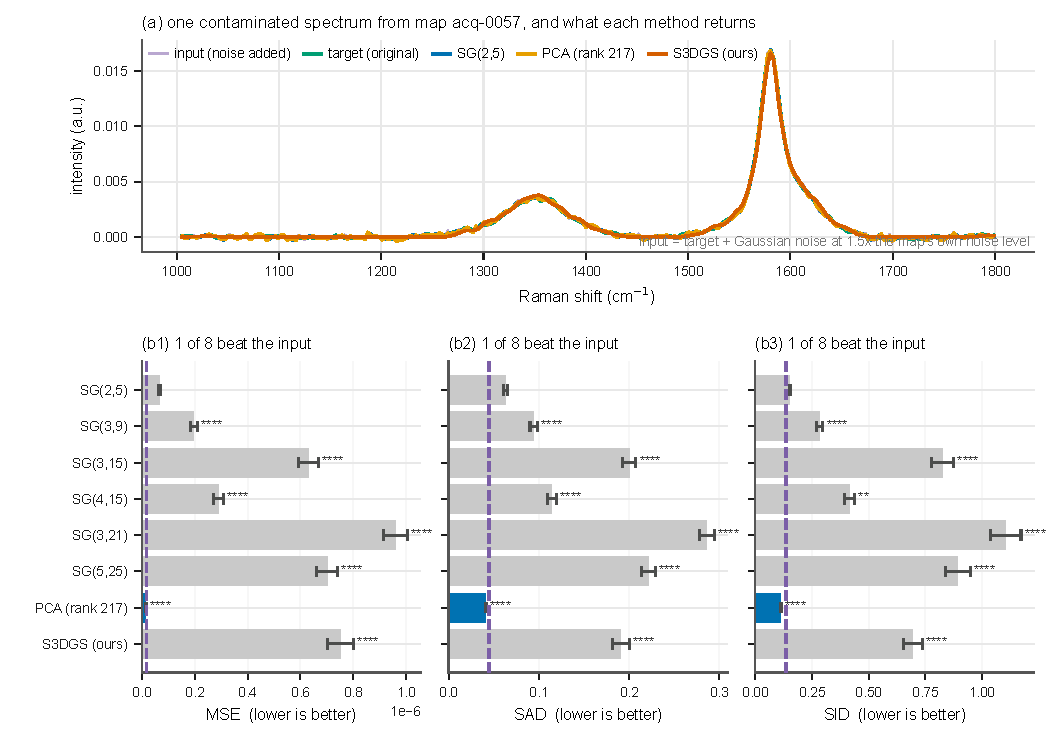
\includegraphics[width=\linewidth]{fig_ml_denoise}
\caption{Denoising benchmark: six Savitzky-Golay filters, PCA truncation
and the fitted Gaussian field. (a) One contaminated spectrum, its target, and
what three of the methods return. (b1 to b3) Mean squared error, spectral angle
distance and spectral information divergence, each a mean over \MLDenoiseN{}
spectra with the standard error of the mean. The dashed line is the noisy
input, so a method is useful only if its bar ends to the left of it; bars are
shaded by whether they do. Stars are a two-sided Wilcoxon signed-rank test
against the best Savitzky-Golay filter, Benjamini-Hochberg corrected.}
\label{fig:mldenoise}
\end{figure*}

\subsubsection{Classification}

The second benchmark asks what a conventional supervised model can recover from
these spectra, and uses it as a probe of the corpus rather than as an end in
itself. We evaluate \MLNmodels{} scikit-learn classifiers
\cite{pedregosa2011scikit}, in the spirit of automated model surveys
\cite{pandala2021lazypredict}, on two tasks with genuine labels.

The first is \emph{particle against substrate}: a segmentation task whose
labels come from an Otsu split on total counts, while the features are
area-normalised spectra. Normalisation removes the intensity difference the
labels were derived from, so a model must learn spectral shape rather than
brightness. The second is \emph{which acquisition configuration produced this
spectrum}. That second task is a diagnostic with real consequences: if a
classifier can identify the recipe from a spectrum, then apparent chemical
differences between samples measured under different recipes may be
instrumental rather than material, which is exactly the confound that
motivates carrying acquisition configuration as a first-class node in the graph
(\S\ref{sec:kg}).

Splits are by \emph{map}, never by spectrum. This matters more than it may
appear. Spectra from one map share a specimen, a focus, a calibration and a
noise realisation, so a random split over spectra would place near-duplicates
on both sides and report an accuracy that reflects memorisation. Held-out maps
are the honest test, and the accuracies we report are correspondingly lower
than a spectrum-level split would produce. A majority-class baseline is
included in the benchmark so the numbers can be read against something.

Results are in Fig.~\ref{fig:mlbench}, and every accuracy below is quoted with
the score of always predicting the majority class, because on an unbalanced
task the raw number carries no information on its own.

On particle against substrate the best model reaches \MLParticleAcc\,\%
(\MLParticleModel), trained on \MLParticleTrainMaps{} maps and tested on
\MLParticleTestMaps{} it had never seen. The majority-class baseline is
\MLParticleBase\,\%, so the best model buys \MLParticleLift{} percentage
points, and \MLParticleBeat{} of \MLNmodels{} models clear the baseline. The
lift is the informative part rather than the accuracy: the labels came from an
intensity threshold and the features are area-normalised, so nothing about
brightness survives into the input. What the models are recovering is a
difference in band shape between the two sides of the split, which is the
spectroscopic content the mask was supposed to have and the reason
\S\ref{sec:masking} orients the mask on band contrast rather than on darkness.

On acquisition configuration the best model reaches \MLConfigAcc\,\%
(\MLConfigModel) across \MLConfigTestMaps{} held-out maps against a baseline of
\MLConfigBase\,\%, a lift of \MLConfigLift{} percentage points, with
\MLConfigBeat{} models clearing the baseline. One caveat belongs with that
number rather than in a footnote: the corpus has \MLConfigClasses{}
configurations, but a split by map leaves only \MLConfigClassesTested{} of them
represented in the held-out set, so the effective test problem is smaller than
the nominal one. Fig.~\ref{fig:mlbench} shows the per-class support so this is
visible rather than implied.

That second result is a warning rather than an achievement, and the contrast
between the two tasks is the finding. A normalised spectrum in this corpus
carries recoverable information about which instrument recipe produced it, at a
rate well above chance on maps the model has never seen. Any analysis that compares samples measured under different recipes is
therefore at risk of attributing an instrumental signature to chemistry. This
is not a hypothetical concern in a corpus assembled over months as recipes were
varied, and it is the empirical justification for carrying configuration as a
node and stamping protocols on metric edges rather than treating either as
bookkeeping.

Models that are quadratic or cubic in the training-set size are fitted on a
capped subsample, and the cap is recorded alongside the score in the released
table, so no comparison is silently unequal.

\begin{figure*}[t]\centering
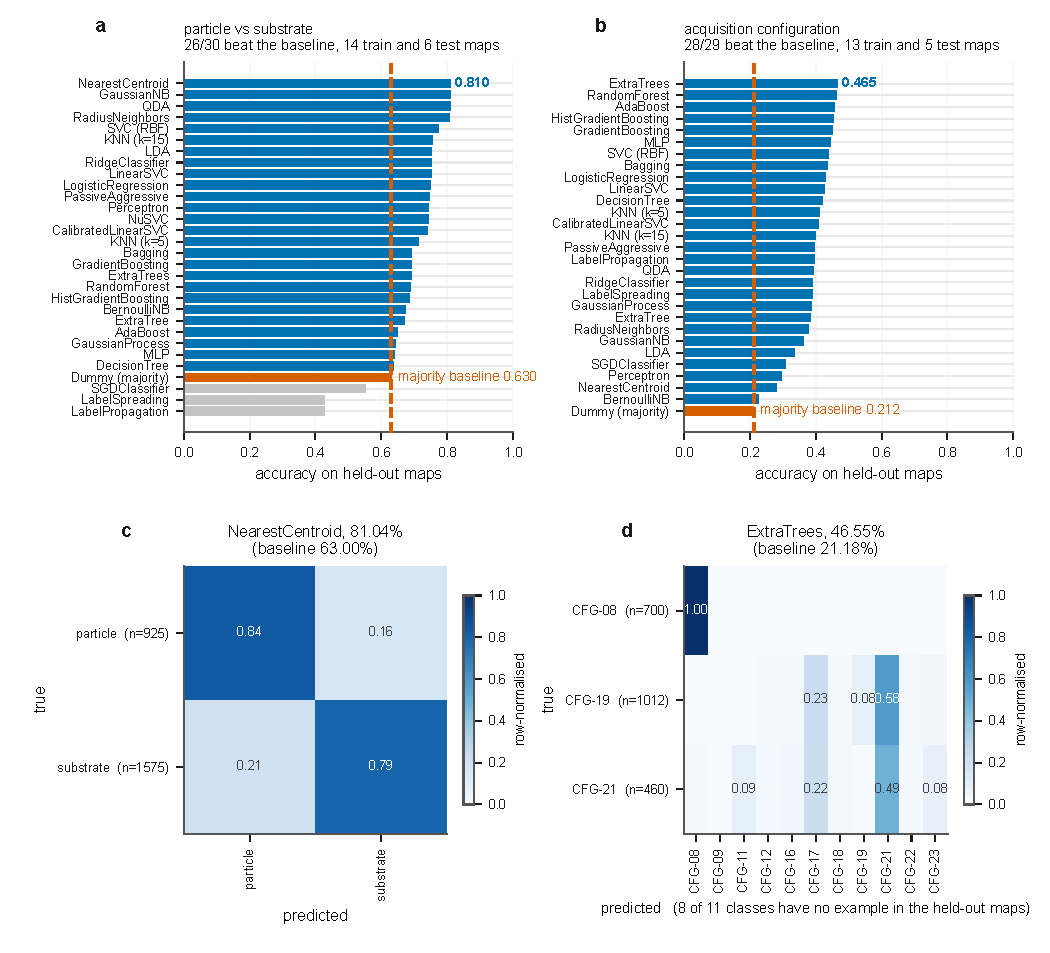
\includegraphics[width=\linewidth]{fig_ml_benchmark}
\caption{Classifier benchmark on map-level splits. (a, b) Accuracy of
\MLNmodels{} models on each task, sorted, with the majority-class baseline
drawn as a dashed line and the baseline model itself in the same colour. Bars
are shaded by whether the model beats that baseline, since accuracy alone is
not interpretable on an unbalanced task. (c, d) Row-normalised confusion
matrices for the best model on each task, with the baseline quoted alongside
the accuracy. Splits are by map throughout, so no spectrum from a test map is
ever seen in training.}
\label{fig:mlbench}
\end{figure*}

% ==================================================================

\subsection{Failure modes encountered}
\label{sec:pitfalls}

Four of the defects we hit produced plausible numbers rather than errors. We
report them because each is a trap the next implementation will meet, and
because the mechanism that caught each one is reusable.

\paragraph{A mask that selected the substrate.}
Particle detection originally took the darker side of the Otsu split as the
particle, which is right for the specimen the rule was written against. On the
wider corpus it is right on some maps and inverted on others, and the failure is
silent in every downstream number: a fit still converges, band maps still look
like maps, and a disorder index still comes out bounded in $[0,1]$. It was found
by plotting measured and reconstructed band maps on a shared colour scale, which
made it visible that the high-signal region sat outside the fitted mask, and
confirmed by measuring band contrast on each side. The correction, orienting on
band contrast (\S\ref{sec:masking}), changed results materially rather than
cosmetically: on one map, held-out PSNR for the same fitting budget moved from
\SI{10.9}{\decibel} to \SI{22.6}{\decibel}, because the field had previously
been spending its primitives on substrate. The lesson we would generalise is
that a rule derived from one specimen's appearance should be replaced by a
measurement of the property actually wanted before it is applied to a corpus.

\paragraph{A truncation box that walked off its own Gaussian.}
The $3\sigma$ box was originally located by dividing the offset from the axis
origin by a median channel spacing. That is correct for a uniform axis. The
fitted wavenumber axis is not uniform: withholding every fifth channel leaves
gaps of $1,1,1,2$ repeating, so the index estimate drifts by about a quarter of
an index per channel and, after sixty channels, the box has left the primitive
it belongs to. The field then loses exactly the contributions nearest each
centre. Nothing raised, the loss still decreased, and the rendered maps still
looked correct. What caught it was comparing the truncated evaluator against
the exact dense one on the same points, which is now a regression test on a
deliberately non-uniform axis.

\paragraph{A similarity threshold that encoded itself.}
Building \code{SIMILAR\_TO} from an absolute cosine cut produced a graph with
communities and a respectable modularity. It was measuring the threshold: at
$0.65$, two thirds of all pairs are linked, because every spectrum in a carbon
corpus has D and G bands. The diagnostic was to plot the distribution of
pairwise similarity before choosing a rule, rather than after.

\paragraph{An anonymisation leak from a derived column.}
The path scrubber worked correctly, and material names still reached the
published tables, because a downstream dictionary mapped anonymised codes back
to human-readable class labels for plotting. Scrubbing inputs is not sufficient
when derived columns can reintroduce what was removed. The gate that now runs
over the outputs also caught a false positive of its own, a five-digit specimen
pattern matching inside a hexadecimal content digest, which is why its
identifier patterns require alphanumeric rather than digit boundaries.

% ==================================================================

\subsection{Discussion}
\label{sec:discussion}

\paragraph{What the reader changes, and why it is a scientific rather than an
engineering point.}
It is tempting to file a binary-format reader under infrastructure. The effect
here is on what could be concluded. With text exports alone the corpus held one
hyperspectral map, the knowledge graph was disconnected, and most curve-fit
tables carried no provenance at all. With the binaries read directly it holds
\Nrawmap{} maps and the graph is essentially connected. Nothing about the
experiment changed; the experiment had always produced this data. What changed
is the selection mechanism between the instrument and the analysis, which was
previously an operator deciding which files to export by hand. Any conclusion
drawn from the exported subset was conditioned on that decision, and the
conditioning was invisible. Community efforts to standardise Raman practice
have concentrated, rightly, on acquisition and preprocessing
\cite{ntziouni2022review,barton2022chemometrics}; the path from instrument
storage to analysis deserves the same scrutiny.

\paragraph{Metrics that measure the instrument rather than the method.}
The clearest methodological result here is negative. Held-out PSNR across our
maps spans more than \SI{16}{\decibel}, which reads as a representation that
works on some data and fails on others. Referred to each map's own measurement
noise, the same fits sit between \SplatResidNoiseMin{} and
\SplatResidNoiseMax{} of the noise floor, which reads as a representation whose
error is set by the acquisitions. The second description is the correct one,
and the difference is not a matter of presentation: the first would lead an
experimenter to tune the model, and the second to lengthen the exposure. We
suspect this confound is common wherever reconstruction quality is reported on
measured rather than synthetic data, and the remedy is cheap, since an
independent noise estimate is available from the spectra themselves.

\paragraph{Interpretability of the primitives.}
Unlike a latent code or a network weight, a fitted ellipsoid has units. Its
wavenumber centre is a band position, its extent along that axis a bandwidth,
its amplitude an intensity, and its spatial semi-axes a domain size. This
places S3DGS closer to physically constrained decompositions
\cite{georgiev2024unmixing} than to generic compressors, and it means the
representation can be inspected for plausibility rather than only scored. We
are deliberate about the limit of that claim: the primitives localise bands,
they do not assign them to chemical species, and the five-component carbon
model \cite{sadezky2005carbon} is not identifiable from these spectra in any
case.

\paragraph{Where the framework sits relative to learned models.}
The dominant use of machine learning in Raman analysis is discriminative,
mapping a spectrum to a class
\cite{luo2022deep,lussier2020deep,ho2019rapid,ralbovsky2020towards}. S3DGS is
generative over a single map and learns nothing transferable between maps: each
field is fitted independently, with no training set and no risk of leakage
between specimens. That is a limitation when many similar maps are available,
and an advantage when they are not, which is the common case in a
materials-characterisation study with a handful of specimens. It also composes
with the discriminative literature rather than competing with it, since a
fitted field supplies denoised spectra and compact per-pixel descriptors that a
classifier can consume. Approaches that shorten acquisition by learning to
reconstruct \cite{horgan2021high} address the same underlying economics from
the opposite direction.

% ==================================================================

\subsection{Limitations}
\label{sec:limitations}

\paragraph{Scale.}
The CPU engine is demonstrated at $10^3$ primitives.
\S\ref{sec:scale} specifies, but does not implement, the GPU path to millions,
and we make no measured claim about that regime.

\paragraph{Vendor coverage.}
\Nlsixfail{} files remain unread, in an older 32-bit container variant that
stores matrices under a different tag. They are almost entirely autosave,
practice and training scratch, so the scientific loss is small, but the number
is large and we quote it rather than the flattering one.

\paragraph{Identifiability.}
Prior work on this corpus established that the instrument's five-band carbon
fit is not identifiable from these spectra: opening the bounds does not improve
the answer so much as change the model. S3DGS reconstructs the \emph{cube}, and
its primitives are band localisers. Nothing here should be read as a claim that
five specific chemical components were resolved.

\paragraph{Statistical power.}
The corpus contains \Nspecimen{} distinguishable specimen codes and
\Nconfig{} acquisition configurations, and \Nfittable{} curve-fit tables carry
no provenance link at all. Community structure and purity are therefore
illustrative of what the method surfaces, not a population-level result about
these materials.

\paragraph{Scope of the noise-floor claim.}
The claim that reconstruction reaches the measurement noise floor is specific
to noise-limited data and to withheld \emph{channels} of a map the field was
fitted to. On a nearly noise-free map the residual is dominated by
representation error and the ratio exceeds one, correctly. The ratio is a
diagnostic of what limits a given fit, not a score to be maximised.

\paragraph{Not a general-purpose denoiser.}
The benchmark of \S\ref{sec:benchmark} shows the field losing to a short
Savitzky-Golay kernel on per-spectrum MSE at full spectral resolution. We
report that because the opposite would have been easy to imply by choosing a
different comparison. The representation is built for compact, queryable,
interpretable reconstruction of a whole map, and it should be adopted for that
rather than as a drop-in replacement for a smoothing filter.

% ==================================================================

% ==================================================================
\section{Conclusions}
\label{sec:conclusions}

We set out to make a months-long Raman mapping study analysable as a whole
rather than a file at a time, and three things were needed.

The first was to stop treating the vendor's format as a boundary. Reading the
LabSpec\,6 container directly, verified bit identical against the instrument's
own export, took the analysable corpus from one hyperspectral map to
\Nrawmap{} and turned a disconnected graph into a connected one. The subset an
operator happens to export is a selection mechanism sitting between the
experiment and its conclusions, and it is worth removing rather than
documenting.

The second was to give the corpus a relational structure. The knowledge graph
makes cross-sample questions expressible, detects duplicate exports that would
otherwise inflate every count, and enforces at the level of data structure the
discipline that \S\ref{sec:prep-variance} argues for: a band ratio travels with
the preprocessing protocol that produced it, and ratios computed under
different protocols are never compared. Building it also required rejecting the
obvious similarity rule, because in a corpus where every spectrum has D and G
bands an absolute threshold measures itself.

The third was Spectral 3D Gaussian Splatting, which gives each map a compact,
differentiable and interpretable representation adapted from scene
reconstruction to a setting with one viewpoint and a physically meaningful
third axis. Each primitive has units and reads as a band at a position with a
width and an intensity. Across \SplatNfits{} maps and acquisition recipes its
held-out error lies between \SplatResidNoiseMin{} and \SplatResidNoiseMax{} of
each map's own measurement noise, at \SplatComprMin{} to
\SplatComprMax$\times$ compression. That is the result we would emphasise, and
it is one a PSNR table alone would have hidden: the reconstruction is limited
by the acquisitions, not by the model, and on the cleanest map the field is
below the noise floor because it declines to encode noise.

We have also reported the four defects that produced plausible numbers rather
than errors, since each cost real time and each will be met again by anyone
building the same thing. The next steps are the GPU backend of
\S\ref{sec:scale}, spectral dictionaries that give primitives physical line
shapes, a single-map rate-distortion sweep, and a neural-field baseline
\cite{mildenhall2021nerf}.



\subsection{Future work}
\label{sec:future}

\paragraph{A GPU backend, and what it would buy.}
The tiled rasteriser of \S\ref{sec:scale} is specified and not implemented.
Beyond speed, the $10^6$ regime changes what the representation can express: at
present a primitive is constrained to be a few voxels wide so that cost stays
bounded, and with a GPU that constraint could be relaxed to let large smooth
regions be captured by few wide primitives and detailed regions by many narrow
ones, which is the adaptive behaviour that makes 3DGS effective in vision
\cite{kerbl20233dgs}. The closed-form gradients derived here become the test
oracle for the autodiff implementation rather than being discarded.

\paragraph{Spectral dictionaries and physical priors.}
Giving each primitive a code over an endmember dictionary, so that the field
value is $\sum_i a_i G_i(p)(\Phi^\top c_i)(\nu)$, would make every ellipsoid
carry a realisable Raman profile rather than a scalar amplitude. The dictionary
could come from VCA \cite{nascimento2005vca}, from a physics-constrained
autoencoder \cite{georgiev2024unmixing}, or from a reference database such as
RRUFF \cite{lafuente2015power}. A stronger variant replaces the isotropic
spectral extent with an explicit line-shape model, Lorentzian for G and
Gaussian for the disorder bands as the instrument's own fitting software
assumes, which would make band width a fitted physical parameter rather than an
emergent one.

\paragraph{A proper rate-distortion study.}
As noted in \S\ref{sec:results}, our compression figures vary across maps that
also vary in difficulty. The correct experiment sweeps primitive count on a
single map, holding the data fixed, to produce a genuine rate-distortion curve,
and repeats it at several noise levels to show where the curve saturates at the
noise floor. This is inexpensive and is the first thing we would add.

\paragraph{Neural-field baselines and hybrid models.}
A Fourier-featured multilayer perceptron mapping $(x,y,\nu)$ to intensity
\cite{mildenhall2021nerf} is the natural learned counterpart and would
establish whether explicit primitives buy interpretability at a cost in
fidelity, or at no cost. A hybrid in which a coarse field is explicit and a
small network models the residual is the obvious third option.

\paragraph{Extending the graph.}
Three extensions follow directly from the schema. Learned node embeddings would
let similarity be defined over provenance and content jointly rather than
content alone. Temporal edges would expose drift, since the corpus spans months
and includes the calibration runs needed to detect it, connecting to the
instrument-stability concerns raised in interlaboratory work
\cite{fornasaro2020surface}. And treating each acquisition configuration as a
design point would turn the graph into the analysis substrate for the
experimental design the corpus was collected to serve, with response variables
computed from cubes rather than scored by eye.

\paragraph{Beyond carbon.}
Nothing in the framework is specific to carbonaceous materials except the
default band windows and the disorder index. The reader, the graph and the
splatting representation apply unchanged to any Raman mapping study, and the
biological and clinical imaging settings
\cite{kallepitis2017quantitative,bergholt2016raman,shipp2017advances} are where
map counts, and therefore the value of a cross-sample view, are largest.

% ==================================================================

\subsection{Reproducibility}

The framework installs as a package and its test suite covers container
round-trips, pipeline determinism, the analytic gradients against finite
differences, the truncated evaluator against the dense one, graph construction,
anonymisation, and the denoising property. The five pipeline stages run end to
end from the raw study directory, and every number quoted in this manuscript is
emitted by the final stage into a macro file from the pipeline's own outputs,
so that no figure in the text can drift from the data that produced it.
Reconstruction metrics can be recomputed from stored fields without refitting,
which is what made adding the noise-floor analysis after the fits a matter of
seconds rather than hours.

% ==================================================================


\section*{Acknowledgements}
% shared content, included by both main.tex and preprint.tex
The authors thank the operators who acquired the measurements analysed here.
No external funding supported this work.

\textbf{Use of AI tools.} An AI coding assistant (Anthropic Claude) was used
throughout the development of the software described here and in the preparation of
this manuscript. Its use covered implementation of the \ramansp{} package and the
pipeline scripts, including the reverse engineering of the vendor container format;
generation of the figures; and drafting and revision of the manuscript text. All
analytical choices, all reported numbers and all conclusions were checked by the
authors against the released code and its outputs, and the authors take full
responsibility for the content of this paper.

\textbf{Author contributions.} S.P. conceived the study, designed and implemented
the framework and the spectral Gaussian splatting method, carried out the
analysis, and wrote the manuscript. J.S.S. contributed to the interpretation of
the results and to revision of the manuscript. Both authors have read and
approved the submitted version.

\textbf{Conflict of interest.} The authors declare no competing financial
interest.


\section*{Data and Code Availability}
% shared content, included by both main.tex and preprint.tex
The \ramansp{} package, the pipeline stages, the anonymity gate and this
manuscript's asset generator are released together at
\url{https://github.com/siddhartha18pahari/RAMANSP}, and every number quoted
above is regenerated by running them. A companion site at
\url{https://ramansp.vercel.app} carries the same material in a browsable form,
including the cross-sample knowledge graph as an interactive view rather than
as the static rendering of Fig.~\ref{fig:kg}, the figures at full resolution,
and this manuscript.

The corpus is distributed in anonymised form only: specimen, material and
configuration identifiers are replaced by opaque codes by a single-pass
scanner, the forward map is written to a private file that is excluded from the
release, and a gate that fails the build on any surviving identifier is run
over everything shareable. Raw vendor binaries are not redistributable and are
not included; the reader that decodes them is.


\section*{Supporting Information}
% shared content, included by both main.tex and preprint.tex
Machine-readable corpus manifest, knowledge-graph export in GraphML with an
interactive browser view, per-map reconstruction metrics and fitted fields,
full classifier and denoiser benchmark tables, and the anonymity-gate report
(ZIP).


\bibliographystyle{unsrtnat}
\bibliography{refs}

\end{document}
